\documentclass[12pt]{article}

\usepackage[utf8]{inputenc}
\usepackage{amsmath}
\usepackage{amssymb}
\usepackage{graphicx}
\usepackage[hyphens]{url} % Allows line breaks in URLs
\usepackage{hyperref}
\usepackage{setspace}
\doublespacing
\usepackage{natbib}
\usepackage{booktabs} % For better table lines
\usepackage{caption} % For table/figure captions
\usepackage[margin=1.25in]{geometry} % Set margins
\usepackage{amsfonts}
\usepackage{xcolor}
\usepackage{footnote} % Better footnote handling
\usepackage{enumitem} % For customizing lists
\usepackage{lipsum} % Placeholder text if needed, good for testing footnotes

% ---- Hyperref Setup ----
\hypersetup{
    colorlinks=true,
    linkcolor=blue,
    filecolor=magenta,      
    urlcolor=cyan,
    pdftitle={Native Representation in State Legislatures},
    pdfpagemode=FullScreen,
}

% ---- Title and Author ----
\title{Section 2 of the Voting Rights Act and Native Representation}
\author{
    Nicholas Eubank\thanks{Assistant Research Professor, Duke University Department of Political Science and Social Science Research Institute.} \and
    Emily Rong Zhang\thanks{Assistant Professor, UC Berkeley School of Law.}
}
\date{\today} % Or use \date{\today}

\begin{document}

\maketitle
\onehalfspacing

\begin{abstract}
\bigskip \singlespacing
\noindent 
We undertake the first systematic, cross-state investigation of the relationship between Section 2 of the Voting Rights Act and Native representation.  Though it is not necessary for Native representation, it remains an important contributor.  It also contributes to packing of Native voters: safe Section 2 districts---in which Native voters constitute a majority---decrease Native influence in surrounding districts. We provide novel empirical support for a longstanding critique of Section 2's focus on minority ability to \textit{elect}, not their \textit{influence}. Because Native communities have relatively small populations, the focus on electability can impose especially harsh trade-offs on influence. 

\end{abstract}

\newpage \clearpage


\section*{Introduction}

Oral argument during the Supreme Court's rehearing of \textit{Louisiana v. Callais} this term confirmed fears among leading commentators that the Court will strike down (or at least significantly cut back on the protections offered by) Section 2 of the Voting Rights Act (``VRA''),\footnote{The fears generated from \textit{Louisiana v. Callais}, a racial gerrymandering challenge to districts drawn to comply with Section 2, are nothing new; scholars have long raised concerns that the racial gerrymandering line of cases are on a ``collision course'' with Section 2. \textit{See, e.g.,} \cite{charles2017race}.} the most significant portion of the Act that remains in effect after the Supreme Court struck down the coverage formula (Section 4 of the Act)---and by extension the pre-clearance regime (Section 5) in \textit{Shelby County v. Holder}.\footnote{570 U.S. 529 (2013).} There is little doubt that such a decision would be transformative for political representation and districting practices.  Whether we are faced with crafting a replacement for Section 2 that is worthy of its legacy, or considering its continued relevance, understanding the significance of Section 2 requires a more fulsome account of how it has shaped representation through its legal constraints on districting practices in the past and present.

Section 2 has no doubt played an important role in enhancing representation of racial minorities\footnote{To be sure, there is a vast literature on the many other effects produced by the Voting Rights Act beyond enhancing minority representation. \textit{See, e.g.}, works on expanded participation of minority voters, including on the closing of racial registration and turnout gaps; \cite{fraga2016examining} (finding that the language minority provisions of the VRA resulted in a significant increase in Latino voter registration and Asian American turnout).} by putting legal limits on practices that have the effect of diluting minority votes: it targets any electoral ``standard, practice, or procedure,'' which includes districting in a biased manner or the failure to district at all (i.e. electing representatives at-large), that prevents minority voters from electing their candidates of choice. The core of any Section 2 violation is the presence of racially-polarized voting, which describes two nested phenomena: first, that the minority group votes cohesively for their candidate of choice, and second, that the majority group cohesively prefers and votes for a different candidate, such that the minority group's preferred candidate is usually defeated. An important, though not exclusive, remedy under Section 2 is to draw or redraw district boundaries so there are sufficient minority voters in the district for them to elect their candidates-of-choice. These are referred to, often, in short-hand as either majority-minority districts or minority-opportunity-to-elect districts. This way, the racially-polarized voting (which was needed to prove liability under Section 2) no longer interferes with the minority group's ability to elect: even if there is racially-polarized voting, the larger number of minority voters in the districts as compared to majority voters results in the election of the minority's candidate-of-choice.

Using new data and analyses, we shed light on Section 2's effects on an understudied racial minority: Native persons.  We investigate the extent to which representation of Native persons in state legislatures remains influenced by districting practices (and are hence by Section 2). We further investigate existing districts for Native vote dilution in order to understand what Section 2 does---and does not---prevent. If legal reforms, at the federal or state levels, are needed to fill the gap left by Section 2, identifying precisely what and where those gaps are is vital.

This paper sits at the intersection of two literatures.  The first, made more urgent by \textit{Louisiana v. Callais}, is one that has long critiqued Section 2's myopic focus on the creation of majority-minority districts. Though Section 2 has been susceptible to many critiques, an important, enduring, and generative strand originating from Lani Guinier highlights the choice that the Act makes to enhance minority voters' ability to \emph{elect candidates} (through compelling the creation of majority-minority districts), which is not the same as, and could produce trade-offs for, minority voters' ability to \emph{influence politics}. \cite{guinier1989keeping,guinier1991triumph,guinier1992representation}, \textit{see, also} \cite{abrams1992relationships,issacharoff2015voting}.\footnote{This is a well-known critique of Section 2 that surfaced many times before in public debate, notably when the Voting Rights Act was renewed.  \textit{See} \cite{persily2007promise}.} The gravamen of the critique is that the focus on creating majority-minority districts may lead to an overall diminishment of minority political influence if it results in voters being so concentrated in a small number of districts that the benefits of increased descriptive representation do not outweigh the cost of lost political influence over legislators in other districts.

Through a series of decisions that the Court made, elevating formalism over functionalism, the critique became more and more true of how the Act operated. \cite{karlan1992rights,pildes2001voting}. One of the most important such decisions involved the rejection of a more functional view of Section 2 that would have allowed plaintiffs to bring suits to create coalition districts, i.e. districts in which voters of different racial minorities would constitute a majority. The critique also became more and more true in light of two empirical regularities that emerged in the last couple of decades. \cite{pildes2001voting}. Social science evidence emerged, over time, showing that many districts did not necessarily require a majority of minority voters in order to elect minority candidates-of-choice. Nevertheless, ``safe'' districts (from the perspective of compliance with the VRA), i.e. districts that have a majority of voters from a single racial minority, became fixtures of districting schemes. \textit{Id.} By investigating where and which districts elect Native representatives in state legislatures, including by taking a close look at majority-Native districts, we are able to evaluate the strength of the tokenism/formalism critique empirically as it applies to an understudied racial minority.  Importantly, we evaluate the validity of an alternative explanation for safe majority-Native districts: racial geography.  Earlier work does not explicitly discuss the possibility that safe districts may be justified on the ground that they are merely products of where racial minorities live (relative to the majority population), likely because consideration of racial and political geography in redistricting did not fully emerge in the literature until the 2010s. \textit{See infra} Section 3.1.

The second literature that we contribute to in this paper is a quite vast one on Section 2's effects on representation of racial minorities, primarily through the creation of mandated majority-minority districts. While this literature furnishes voluminous evidence on how Section 2 enhanced the political representation of racial minorities, that literature is based primarily on the experience of Black and to a lesser extent on Latino voters.  Though it is possible, if even likely, that these dynamics in the literature are equally applicable to Native voters, any extension is assumed rather than proven.  We thus contribute missing and current analyses on the relationship between districting and the representation of Native persons to this literature.

That literature can be divided into two subsets, each relating to a voting structure that Section 2 reforms.  The first subset, one that we do not directly engage with, concerns the conversion of at-large voting schemes to districted elections (with newly created majority-minority districts) that Section 2 mandates.  Because when there is highly racially polarized voting, at-large voting schemes can prevent minority voters from electing any candidates of choice, Section 2 intervenes in these instances to require that at least some elected offices be elected from districts, and that those districts be drawn in a way that allows minority voters to elect their candidates of choice.  At-large voting schemes were and remain quite common, especially in local governments.  And the literature resoundingly makes clear, based largely on the experiences of Black (and to a lesser extent Latino) voters, that Section 2 mandated or encouraged conversion from at-large to districting schemes have helped significantly increase the number of minority representatives elected (sometimes referred to as descriptive representation). \textit{See, e.g. }\cite{davidson1981atlarge,engstrom1981election,karnig1982electoral,meier1984impact,bullock1993election,marschall2010new,trounstine2008representation}.

The second subset, the one that we directly engage with, concerns Section 2's intervention in how districts in existing districted schemes, like those for Congress, state legislatures or local districted races, are drawn.  Within districted schemes, when the majority voters outnumber minority voters and there is racially polarized voting, minority voters are also unable to elect their candidates-of-choice.  Section 2 thus requires that districts be drawn to allow minority voters to elect their candidates-of choice.  Here, too, majority-minority districts are also typically what are mandated under Section 2.  This literature has similarly found that majority-minority districts have produced tremendous gains in descriptive representation.\footnote{\cite{grofman1989minority,grofman1991impact,sass1995voting,grofman2000drawing,lublin2009has,lublin2020minority}.} This conclusion continues to be reinforced in the literature even as new data and techniques have emerged to assess districting practices more systematically and rigorously. For instance, \cite{chen2021race} deploy a randomized redistricting algorithm and find that failing to district in the race-conscious manner as required by Section 2 would result in a diminution of minority ability-to-elect their preferred candidates in the current era.\footnote{\cite{kuriwaki2023geography} provide the behavioral companion piece to \cite{chen2021race}, assessing the extent of racially polarized voting of different racial groups across the country, and demonstrating the still pervasiveness of racially polarized voting with geographic specificity.} \textit{See, also} \cite{katz2005documenting}.

The ability-to-elect of Black and sometimes Latino voters to elect representatives is usually the main outcome of study in the studies that reach these conclusions. Representation of Native individuals is not usually included in systematic studies of representation across states and contexts. Why not? Perhaps because Native persons constitute, as a purely numerical matter, an ultra-minority.\footnote{\cite{zhang2020native}.} For redistricting to influence representation in the presence of racially-polarized voting, a minority group has to be able to at least come close to constituting a majority in the districts in question. And while this is true in some state legislative districts, especially in the Mountain West and in state houses, it is not true for any congressional district in the country. Given the academic literature's (and political discourse's) focus on \textit{congressional} redistricting,\footnote{\textit{See, e.g.}, \cite{grofman1989minority}; \textit{see also supra} note 6.} Native representation can often be excluded from analyses by design: congressional districts are simply too large for Native populations in any part of the country to come close to a majority. Yet even when studies have considered state legislative redistricting, Native representation is not always included alongside similar analyses for Black and Latino representation,\footnote{\textit{See, e.g.}, \cite{lublin2020minority}.} perhaps because the number of state legislative representatives elected from majority Native districts is small by comparison with other racial groups. Perhaps for this same reason, Asian-American representatives have not typically been included in these analyses either and have required their own separate treatment. \textit{See }\cite{lublin_wright_2024}.

Though one could assume that the many conclusions drawn from the literature on minority representation based on representation of Black and Latino individuals are also true of Native representation as well, doing so would require inferential leaps or untested assumptions. Even in the existing literature, evidence suggests that Section 2 had heterogeneous effects among different racial minorities.  For instance, \cite{stephanopoulos2016race} found that Section 2 had different effects on Black as compared to Latino descriptive representation.  (Indeed, it also found differences between Black descriptive representation in the South and otherwise.)  Whether redistricting has and continues to aid Native representation is its own empirical question that deserves its own empirical investigation. While vote dilution of Native voters comes under the protection of the Voting Rights Act, it is possible that representational gains for other racial minorities are not replicated for Native voters in many circumstances. Section 5 of the Voting Rights Act, the provision that prevented retrogression, only applied to jurisdictions covered by the formula in Section 4 of the Act. Among states with significant Native population, only some were covered jurisdictions.  Moreover, while Section 2 of the Voting Rights Act provides another independent legal provision for preventing Native vote dilution, it is enforced only through affirmative litigation. Given the high costs of Section 2 litigation, \cite{elmendorf2015administering}, we do not know whether affected Native voters were always able to bring meritorious cases challenging vote dilution under the Act, let alone prevail on them.

Though systematic evidence on Native representation is sparse, there is plenty in the literature to suggest that at least some dynamics described in the literature on representation of racial minorities as a whole apply or are similar for Native persons. Though the Native voting rights literature is a relatively small one, it can be described as deep (as opposed to wide): there are important works by scholars and lawyers that document, abundantly and exhaustively, the various obstacles that Native persons faced in seeking political empowerment and representation.


As an initial matter, the literature makes clear that combating vote dilution is only one among many challenges that Native voters face. For instance, \cite{schroedel2020voting} describes a variety of historic and current vote suppression and abridgement issues in Indian Country (e.g., language barriers, voter identification laws, long travel times to vote) alongside vote dilution issues. Historic and ongoing problems that Native voters face in exercising their right to vote (succinctly described as vote denial, \cite{tokaji2006new}, are of course deeply intertwined with vote dilution; both are strategies to reduce the political power of Native persons.

Among the plethora of obstacles that the literature documents, vote dilution through districting practices stands out as an important and historic obstacle to Native political empowerment—and to representation of Native persons and interests. Several important books have been written on the topic of Native voting rights, and the struggle to be represented, whether produced by at-large voting schemes or through biased district lines, is always included and addressed in each of them. Because these books tend to address lawsuits brought pursuant to Section 2 of the VRA, and because Section 2 claims necessitate an ``intensely local appraisal,''\footnote{\textit{Thornburg v. Gingles}, 478 U.S. 30, 78 (1986) (citation omitted).} they tend to discuss vote dilution—and the transformative effect that these suits have had on enhancing Native representation within the particular contexts that gave rise to those suits.

To be sure, the purpose of these books has not been to provide a systematic study of all districts at a certain level of government that affect Native persons, but rather to analyze the conditions that give rise to legal challenges and to consider the effects that successful suits have had on representation. But they nevertheless allow us to draw some context-limited but important conclusions: at-large schemes have played an important one in thwarting the election of Native representatives (preferred by cohesive Native voters) in at least a non-trivial number of instances, and that the successful election of many Native representatives can be attributed to the introduction of single-member districts. In brief, redistricting has mattered for producing or enhancing Native representation. \cite{mccool2007native}'s canonical book on Native voting rights and the Voting Rights Act canvassed all voting rights litigation brought by or on behalf of Native voters; among them, suits challenging vote dilution through districting practices are legion.\footnote{For the impressive catalogue of all cases, \textit{see} \textit{id}. at 48-68.} Indeed, they found that suits challenging at-large electoral schemes constitute ''the largest category of voting rights cases in Indian Country.''\footnote{\textit{Id}. at 75.} \cite{mcdonald2010american}'s book is a collection of specific Section 2 Native vote dilution cases, spanning states including Montana, South Dakota, Colorado, Nebraska, and Wyoming and governments including school districts, city commissions, county commissions, and state legislatures. Through these cases, we see that conversion from at-large schemes or redrawn district lines produced many improvements to Native representation.

Yet these important contributions still leave many questions unanswered. Even if it can be assumed that Native representation, like representation of other minorities, has been enhanced by race-conscious districting, exactly where and how much representation has been enhanced or stymied by recent redistricting efforts remains uninvestigated. Perhaps more importantly, these contributions derive from facts and cases from a much earlier era of Section 2 enforcement when the provision first applied to Native persons. We know little, systematically or not, about the current relationship between Native representation and districting. And yet this question, of how much Section 2 and its legal constraints on districting practices currently is or is not relevant for Native representation, is one that is all the more important to pose and answer given the jeopardy that Section 2 itself is in.

The goal of this paper is thus to undertake a dedicated, systematic, and localized analysis of redistricting's current impacts on Native representation at the highest level of districting where it matters (state legislative districts). It assesses districts drawn in the most recent redistricting cycle (based on the 2020 decennial census) as well as the one immediately preceding it (based on the 2010 decennial census) for the simple reason that little is known about these districts during this time period. This paper investigates only state legislative districts and not sub-state levels of representation (e.g. city councils or county commissions) because of the relative ease of data collection: boundaries of state legislative districts are collected by the census bureau and are readily available to researchers, whereas local government district boundaries must be collected individually.

Conclusions drawn about the relationship between districting and Native representation from this paper are limited to the particular context—state legislative districts—that this paper investigates. There is strong reason to believe that Native representation at the sub-state and local levels are intimately tied to districting practices and it is possible that districting impacts local representation in different and more powerful ways.\footnote{It is possible that sub-state and local levels of districting produces ``second-order'' diversity, \cite{gerken2005secondorder}, a dynamic we are not able to explore. Another important way in which sub-state and local offices may interact with state legislative offices (and those at the statewide and national levels) is that office-holding at lower levels of government may ``build the bench'' for higher offices, \cite{greenwood2016fair} at 212-13 (presenting statistics on Black, Hispanic, and Asian representatives in Congress who started their careers in local government), a dynamic that we also do not explore here.} Researchers have demonstrated that districting reforms have led to enhanced local representation for other minority groups. \textit{See, e.g., }\cite{shah2013are} (demonstrating the strong effect that the VRA has had on Black representation in city councils throughout 1979-2001); \cite{marschall2010new} (finding similar effects for Black representation on school boards as well). And there are strong reasons to believe that local Native representation especially benefited from reforming redistricting practices. \cite{mccool2007native} document the election of many first Native officials in a variety of local governments (e.g. county commission of San Juan County (New Mexico), San Juan County (Utah), Big Horn County, Roosevelt County, Rosebud County, Blaine County (Montana); school districts in Navajo County (Arizona), New Mexico). Future work on Native representation at the sub-state levels is therefore both sorely needed and likely to reveal large effects of redistricting.

This paper proceeds in three parts. In the first part, to determine how much districting still matters for Native representation, we ask where Native state legislators (and congresspersons) are elected from. We learn that Native representation today does not rely solely on majority-Native districts. (The implication here is that there is not sufficient levels of racially-polarized voting to defeat the election of these Native representatives.) But several states, especially those in the Mountain West, still primarily elect Native representatives through majority-Native districts. The second part investigates the majority-Native state legislative districts that elect Native representatives. We learn that though not universally the case, many of these Native ability-to-elect districts comprise significant Native population (often over 70\% of the districts' population). Combining lessons from the first two parts of the paper, we find that Native representation seems to have a paradoxical reliance on Native district composition: Native representatives are elected at far higher \emph{rates} in majority-Native districts, but because majority-Native districts are relatively rare, \emph{proportionally} more Native representatives are elected from non-majority Native districts. In the remainder of the paper, we zero in on majority-Native districts because of concerns that there may be vote dilutive effects from districts with high concentrations of Native voters (conventionally described as ``packing,'' where the minority group is too concentrated within certain districts). The third part of the paper tests for the presence of vote dilution more formally by applying a measure called ``dislocation,'' adapted from the context of partisanship to the race context. Vitally, this measure takes into account the racial geography (where Native and non-Native populations live) of the relevant districts. We find evidence that at least some majority-Native districts are descriptively, if not legally, packed. We also find evidence that there are Native populations in non-Native-majority districts that are descriptively cracked. These observations lead us to conclude that though Section 2 has continued relevance for Native representation, it leaves some Native vote dilution effects unresolved.

\section{Where Section 2 Matters for Native Representation (and Where it Does Not)}

Despite the relatively thin literature on Native representation through redistricting, the raw data shows that the improvements in Native representation have been no less dramatic than those of other racial groups.\footnote{Our consideration of Native representation in this section is entirely limited to the election of Native representatives. To be sure, non-Native representatives may be preferred by Native voters, and Native representatives may not be the most preferred candidate by Native persons. But by and large, Native representatives tend to be selected from majority-Native or near-Native-majority districts, indicating a general preference by Native voters to elect Native candidates when they have sufficient voting strength to do so. And it makes sense to start by understanding descriptive representation if only because identifying substantive representation is significantly more challenging. It would require highly contextualized analyses of voting patterns and elections data. To the extent that the literature would be advanced by understanding if and when descriptive and substantive representation clash, getting a sense of where descriptive representation is occurring lays the foundation for that future work.} Even though data sources on Native state representatives are lacking (especially from prior decades, with only aggregated data from a few discrete points in time), progress has clearly been nothing short of monumental. \cite{reingold2019gender}'s exhaustive study of gender and race/ethnicity representation in state legislatures shows that between the mid-1990s and 2018, the number of Native American state legislators went up from 26 (0.3\% of state legislators) to 81 (1.1\%). \cite{blasingame2025are}'s more recent study on the legislative activities of Native legislators collected additional data on the number of Native legislators elected since 2018 (till 2023); those numbers are substantially similar ($\sim$81); \textit{see also id.}, Figure 1, for histogram of Native state legislators elected between 1993-2023.\footnote{As an initial project to investigate Native representation, our paper necessarily omits other aspects of Native representation that have long been identified in the literature as vital to the representation of racial minorities' political interests.  One central dynamic that we do not investigate, for instance, is Native representatives' ability to govern once they are elected to office. \textit{See} \cite{karlan1993rights} For work done to investigate these dynamics for other racial minorities, \textit{see, e.g.,} \cite{hutchings2004congressional}.}

Among the many reasons for such progress is surely the passage of the Voting Rights Act.\footnote{To be sure, specific quantitative causal evidence for the Voting Rights Act's contribution to enhanced Native representation is wanting. But given the vast literature on the VRA's effects on enhanced representation of other racial groups, and that improvements in Native representation occurred on the same trajectory as those of other racial groups, it is clear that the VRA is responsible for much of the improvement in Native representation.} But legal change is also not solely responsible. While slow, attitudinal changes are surely also contributing to enhanced Native representation. To be sure, pitched racially polarized voting between white and Native voters is still a reality in some places and in some elections.\footnote{\textit{See} \cite{zhang2020native}, for a discussion of an extreme example of modern racially polarized voting between white and Native voters in San Juan County, Utah.} But at least in certain political contexts, there is evidence that erosion of racial prejudices is contributing to enhanced Native representation. Native representation in Congress in the modern era reveals the power of attitudinal change, as opposed to districting reform, in electing Native representatives. Numerous Native representatives have been elected to statewide and national offices\footnote{The most authoritative source on Native congresspersons is a memo that the Congressional Research Service published on the subject in 2013. \cite{crs2013members}. As our correspondent at the CRS helpfully noted, the memo does not include a couple of notable additions from 2019: Representatives Sharice Davids (D) (Kansas, CD 3) and Deb Haaland (D) (New Mexico, CD 1) (who later served as Secretary of the Interior).} (e.g. Colorado Senator Ben Nighthorse Campbell from 1993-2004; Kansas Representative Sharice Davids since 2019). These Native representatives could not have been elected to office without relying on crossover voting (i.e. white voters voting for Native representatives), as votes from Native voters alone were insufficient to elect these representatives.\footnote{Native representation in Congress is also not a uniquely modern phenomenon; since 1870, Native persons have served in Congress, representing large congressional districts and sometimes entire states, albeit in very small numbers. \textit{See, id.}}

While the purpose of this paper is not to evaluate the extent of racially polarized voting, vital as that work might be, it acknowledges that districting may not always be relevant for the election of Native representatives. Learning where Native state representatives are elected from can help us identify where representation is likely occurring without the help of districting—and also where representation is likely very much dependent on districting. And identifying the extent to which districting matters is vital to understanding the import of Section 2 of the Voting Rights Act, because that is the central mechanism by which it intervenes to enhance minority ability-to-elect.

Table \ref{tab:states_electing_native}, below, shows 1) which states Native representatives were elected from in 2023, the last year in which we have available data and also the high watermark for election of Native representatives\footnote{These data are from those collected for \cite{blasingame2025are}, replication archive.} and 2) the state's Native percentage of the population (sorted in ascending order):\footnote{These data for all states except Hawaii are based on any-part Native populations from the 2020 census compiled by \cite{ncai2021overview}. Because Native Hawaiians are given a separate racial category in the census, the figure for Hawaii is based on the percentage of Native Hawaiians in the state. See \cite{oha2024census}.}

\begin{table}[ht]
\centering
\caption{States electing Native representatives}
\label{tab:states_electing_native}
\begin{tabular}{lcc}
\toprule
State & Legislators & \% Native \\
\midrule
Mississippi    & 1 & 1.8\% \\
New Hampshire  & 1 & 1.8\% \\
South Carolina & 1 & 2.1\% \\
Tennessee      & 1 & 2.3\% \\
Minnesota      & 5 & 2.8\% \\
North Carolina & 2 & 3.0\% \\
Nevada         & 1 & 3.4\% \\
California     & 1 & 3.6\% \\
Kansas         & 2 & 3.8\% \\
Washington     & 4 & 4.1\% \\
Oregon         & 2 & 4.4\% \\
Wyoming        & 1 & 4.8\% \\
Arizona        & 5 & 6.3\% \\
North Dakota   & 2 & 7.2\% \\
Montana        & 11 & 9.3\% \\
South Dakota   & 4 & 11.1\% \\
New Mexico     & 8 & 12.4\% \\
Oklahoma       & 12 & 16.0\% \\
Hawaii         & 13 & 21.8\% \\
Alaska & 8 & 21.9\% \\
\bottomrule
\end{tabular}
\end{table}

This table shows that Native legislators are elected from a large variety of states, 20 in total. Some of these states with large Native populations, like Hawaii and Alaska, are perhaps unsurprising. Others, especially states with small Native populations, are perhaps more surprising. The table also shows that the absolute number of Native representatives at the state legislative level is not large; many states, especially those with small Native populations, elect some but very few Native representatives.

What dynamics give rise to the election of Native representatives in these states? Are those dynamics uniform or different across state contexts? More precisely, what role does districting play in the election of these Native representatives? If districting—and the demographic composition of the districts—is contributing to the election of Native representatives, then Section 2, by extension, likely plays a direct role. But it could be the case, as with the election of Native congressional representatives, that the election of some of these representatives cannot be directly attributed to Section 2. Though Section 2 nominally applies to all states and all redistricting schemes, it does not functionally apply unless certain necessary predicates are met: the three \textit{Gingles} preconditions as set out by the Supreme Court's decision in \textit{Thornburg v. Gingles}. The first Gingles precondition is that the Native population must be ``sufficiently numerous and compact to constitute a majority'' in a state legislative district. That condition likely cannot be met in many of these states either because there simply are not enough Native persons in the state to begin with, or even if there are enough to constitute a majority in a state legislative district, the Native population is distributed in such as a way that they cannot be drawn into a compact district in which they constitute the majority. And if these representatives are elected from districts with a small percentage of Native constituents, that would indicate the presence of significant white cross-over voting, at least in the parts of the state that elects these representatives, and thus a lack of racially-polarized voting, the second and third Gingles pre-conditions for establishing Section 2 liability. If representatives are successfully elected from districts in which Native persons do not constitute a majority, their election must be supported by significant or even overwhelming vote shares from white voters.

To investigate the role that districting plays in electing these representatives, Table \ref{tab:native_vap_by_state} compiles the mean demographic composition of the districts in each state that elects Native representatives. Specifically, it presents what percentage of the district is comprised of Native voters, i.e. the percentage Native in Voting Age Population,\footnote{It is custom to evaluate demographic composition of districts using the Voting Age Population (as obtained from Census PL 94). The Voting Age Population is the population in the district over the age of 18 (the age at which one attains the right to vote).} ``VAP''. The table is sorted in ascending order of mean percentage Native VAP:

\begin{table}[ht]
\centering
\caption{Native VAP in Districts Electing Native Representatives by State}
\label{tab:native_vap_by_state}
\begin{tabular}{lr}
\hline
 State          &   Mean Native VAP \\
\hline
 Mississippi    &                3\% \\
 New Hampshire  &                2\% \\
 South Carolina &                1\% \\
 Tennessee      &                2\% \\
 Minnesota      &                5\% \\
 Hawaii         &                3\% \\
 North Carolina &               47\% \\
 Nevada         &                2\% \\
 California     &                3\% \\
 Kansas         &                6\% \\
 Washington     &                3\% \\
 Oregon         &                4\% \\
 Wyoming        &               36\% \\
 Arizona        &               20\% \\
 North Dakota   &               49\% \\
 Montana        &               41\% \\
 South Dakota   &               54\% \\
 New Mexico     &               36\% \\
 Oklahoma       &               16\% \\
 Alaska         &               62\% \\
\hline
\end{tabular}
\end{table}


The table shows that there is significant variation in which states rely on majority-Native districts to elect their Native representatives.\footnote{An important and uninvestigated assumption that we make here is that Native voters by and large vote cohesively for these Native representatives, and given their numbers in these districts, they can successfully elect these candidates of choice. Given that in these states, Native representatives are not usually elected except in districts with a large percentage of Native voters, it is probably the case that at least some significant portion of Native persons in these districts vote cohesively for the Native representatives. To be sure, the relative extent of racially-polarized voting in these districts likely varies.} The states might appropriately be divided roughly in descending order of how much districting (and Section 2) matters into three sets.

The first set of states, California, Kansas, Minnesota, Mississippi, New Hampshire, Nevada, Oregon, South Carolina, Tennessee, and Washington, are states with relatively small Native populations and which elect Native representatives from districts with small Native VAP percentages.  These are states in which districting likely does not contribute much to Native representation. And by extension, the Native representatives they elect cannot be directly attributed to Section 2. For instance, California is home to by far the largest number of Native persons in the country, but because the state is so populous, Native persons constitute only 3.3\% of the total population. And given the way that the Native population is distributed across the state, Native persons cannot constitute a majority in even state assembly districts (the smallest state legislative district). Indeed, the California state house district with the highest proportion of Native persons is only about 8\% Native. Given the demographics of the surrounding area, there is no reason to believe this could be increased by redrawing the district in a reasonably compact way. To be sure, some other states in this group have more significant proportions of Native persons within the state. Utah, for instance, has a state house district that is 22\% Native. But the same point holds across all of these states: while they have a non-trivial proportion of Native persons in the state, the numbers (and the geography) simply do not give rise to the first \textit{Gingles} precondition, requiring that the racial minority be ``sufficiently large and geographically compact to constitute a majority'' in even state house districts. If the first \textit{Gingles} precondition is not met for state legislative redistricting, Section 2, though facially applicable to these states, does not functionally apply for these districts.

The second set of states, Oklahoma and Hawaii, are similarly states in which districting likely does not contribute much to Native representation. But they are different because they have significant Native populations. Indeed, they have some of the highest percentage of Native persons in the country. And they elect many Native representatives. These are states in which the first \textit{Gingles} precondition can easily be met with respect to at least some state legislative districts. But they are states in which evidence of the second and third \textit{Gingles} preconditions are sparse, judging by the successful election of Native representatives from districts in which Native populations are far from the majority. In Hawaii, the mean Native percentage across the districts electing Native representatives is 2.3\%; the max is 4.6\%. The numbers are higher in Oklahoma but still relatively low in absolute terms: the mean Native percentage across districts electing Native candidates is 10\%; the max is 19\%.\footnote{Hawaii elects proportionally more Native representatives than Oklahoma does, even if Oklahoma elects more in absolute numbers, because Hawaii has many fewer state representatives in total compared to Oklahoma. In 2019, 13\% of Hawaii's state legislative representatives are Native, and 9\% of Oklahoma's representatives are Native. Both elect a smaller proportion of Native representatives than their state's proportion of Native persons.} The dynamics in these states illustrate how voter behavior can overcome geography and demographics. As long as voters are willing to vote for Native candidates (and by extension Native-preferred candidates), Native voices can be present in the legislature.\footnote{A closer look at these states, and those described in the first set, reveals some fascinating dynamics of partisan and racial politics behind Native representation more generally (that are also unfortunately not the focus of this paper). As a general matter, Native representatives tend to be Democratic. Among the 82 Native representatives in office in 2019, 16 were Republican and 1 was undeclared; among the 15 Native representatives in office in 2019 in the purple states, 2 were Republican. Most of the Republican Native representatives are from Oklahoma. Democratic Native representatives (outside of the Midwest) tend to identify also with another race. In the South, they often also identify as Black (\textit{see, e.g.}, Representatives Reginald Meeks from Kentucky (HD 42) and Talmadge Branch from Maryland (HD 45)). In the West, they also often identify as Latino (\textit{see, e.g.}, Representatives Todd Gloria (HD 78) and James Ramos (HD 40) from California and Angela Romero from Utah (HD 26)). (We rely on what representatives self-describe in either their campaign or official websites and through their membership in race-identifying legislative caucuses.)}

The last set of states are those where demographics and political geography–and by extension districting–are probably still of enduring importance to Native representation. They can be subsetted further based on the size of the Native population in the states into two subsets: those with a significant Native population (Alaska, Arizona, Montana, New Mexico, North Dakota, South Dakota, and Wyoming) and a single state that does not (North Carolina). Though districting likely matters for all of these states in electing their Native representatives, it is less significant in North Carolina for the simple reason that the Native population in the state is relatively small, around 3\%. Therefore, though the Native population in North Carolina is ``sufficiently numerous and geographically compact to constitute a majority'' in a state house district, it is not sufficiently numerous to constitute a majority in more than a single state house district (or a single state senate district).

By contrast, the other states are those with some of the highest proportion of Native persons in the country,\footnote{The mean Native percentage in these states is around 10\%, although the mean is significantly affected by Alaska, which is about 21\% Native. Among the others, the mean Native percentage is 7.6\%.} elect a large proportion of the country's Native representatives, and appear to do so because of how districts electing these representatives are drawn. Simply put, these are states with significant Native representation that would be at stake if Section 2 were struck down or modified. The still heavy reliance on majority-Native districts to elect Native representatives in these states may also be connected to a troubled history with Native tribes and population within their states. Many of these near majority-Native districts were the hard-won result of protracted Section 2 litigation in decades past. \textit{See} \cite{mcdonald2010american} (describing litigation in Montana, South Dakota, and Wyoming, among other states); \textit{see generally} \cite{mccool2007native}. And as the litigation revealed in great detail (not only of racially-polarized voting but also of the Senate Factors), many egregious historical and current conditions interacted to produce significantly diminished opportunities by Native persons to elect their candidates of choice in these states and regions.\footnote{\textit{Id}.}

That the fate of Native representation is still intimately bound up with political geography and demographics in these states is why we focus the rest of the paper on them. For efficiency, we refer to them as the ``study states.'' Put in concrete terms, if Section 2 is struck down or modified, it is representatives in the study states who may be affected. But to what extent?  Though we know that districting likely matters for electing Native representatives, one central question we must ask to better understand the stakes of the decision in \textit{Louisiana v. Callais} is: \textit{how much} does districting matter in these states for electing Native representatives?

\section{Native Ability-to-Elect}

To better understand the role that Section 2 plays in these states, we next ask what circumstances give rise to Native voters' ability to elect Native representatives.  We do so by investigating the racial composition of state legislative districts in these states.  What do the districts electing Native representatives look like in the study states?  Knowing these empirical patterns will help us understand how reliant Native ability-to-elect is on how districts are drawn.  We first gather descriptive data on the racial composition of districts electing Native representatives.  Then, we use the data on the racial composition of districts and whether Native representatives are elected to estimate what percentage Native a district has to be in order to elect a Native representative.

\subsection{Racial Composition of Districts Electing (and Not Electing) Native Representatives}

The relationship between Native representation and districting is one of contradictions: Native representation relies heavily on both districts with few and many Native persons.  Native representatives are elected at far higher \emph{rates} in districts that have larger Native Voting Age Populations (VAP)\footnote{It is custom to evaluate demographic composition of districts using the Voting Age Population, i.e. total population of individuals over the age of 18 (as obtained from Census PL 94).}, but because districts with high Native VAP are relatively rare, proportionally more Native representatives are elected from districts where the majority of the VAP is not Native. 

This dual reality is illustrated in Figure~\ref{fig:Bar_NVAP_ElectNR} below. This bar chart plots the distribution of districts that do (and do not) elect Native representatives by districts' Native VAP for all state legislative districts from 2022 in the study states.\footnote{Data on Native representation comes from \cite{blasingame2025are}. Results are shown for 2022 electoral districts, Native representation is measured in 2022 and 2023, and demographic data comes from the 2020 census. Results are similar for 2012-2020 districts using data from the 2010 census and looking at whether a district has elected a Native representative any point during that period.}

\begin{figure}[h]
  \centering
  
\includegraphics[width=0.8\textwidth]{figures/district_native_share_hist_2020.png}
  \caption{Districts electing (and not electing) Native Representatives by Native VAP}
  \label{fig:Bar_NVAP_ElectNR}
\end{figure}

The fact that Native representatives are elected at higher rates in districts with higher Native VAP is immediately evident from the fact that a larger proportion of districts with high Native VAP (those on the right side of the figure) are blue, meaning they have elected a Native representative. The districts with low Native VAP on the left, by contrast, are almost entirely orange. Indeed, in districts with less than 10\% Native VAP (the left-most bar in the figure, which has been truncated for readability), only \input{stats/num_leftbar_dists_native_2020}of \input{stats/num_leftbar_dists_total_2020}districts have elected Native representatives, a rate of only \input{stats/share_leftbar_dists_native_2020}\unskip\%.

At the same time, however, this figure also makes it clear that the vast, \emph{vast} majority of districts have very low Native VAPs. As a result, while it is true that Native representatives are elected at a much higher rate from majority Native districts, a huge proportion of elected Native representatives come from districts that are not majority Native VAP. Indeed, \input{stats/share_native_districts_over50_2020.tex}\unskip\% of districts that elected a Native representative during this districting cycle in our sample were elected from districts that had Native VAPs less than 50\%.\footnote{Results are similar for the last redistricting cycle — \input{stats/share_native_districts_over50_2010.tex}\unskip\% of districts that elected a Native representative between 2012 and 2020 were elected from districts with Native VAPs of less than 50\%.}

This apparent contradiction is often — but not always — evident when we separate our analysis by state, as shown in  Figure~\ref{fig:Bar_NVAP_ElectNR_bystate}. In states like South Dakota, Arizona, and New Mexico, it is clear that while the rate of Native representation are higher at higher Native VAP, many Native representatives come from districts with low Native VAPs. In states like Wyoming, Alaska, or most dramatically Montana, if districts that were predominantly or majority Native VAP were to disappear, the consequences for Native representation could be more dire. Indeed, \input{stats/share_native_districts_over40_MT_2020.tex}\unskip\% of districts that have elected Native representatives in Montana had Native VAP of 40\% or more.

\begin{figure}[htbp!]
  \centering
  
\includegraphics[width=0.8\textwidth]{figures/district_native_share_hist_2020_bystate.png}
  \caption{Native VAP \& Probability of Electing Native Representatives (by State)}
  \label{fig:Bar_NVAP_ElectNR_bystate}
\end{figure}
\pagebreak

This complexity makes clear why predicting the exact effect of Section 2 on Native representation is difficult. Even in these states where Section 2 is functionally operative, none of the states rely entirely on majority-Native districts (or even near majority-Native districts) to elect their Native representatives.\footnote{An important and untested assumption that we make here is that Native voters by and large vote cohesively for these Native representatives, and given their numbers in these districts, they can successfully elect these candidates of choice. Given that in these states, Native representatives are not usually elected except in districts with a large percentage of Native voters, it is probably the case that at least some significant portion of Native persons in these districts vote cohesively for the Native representatives. To be sure, the relative extent of racially-polarized voting in these districts likely varies.} These states elect many Native representatives from districts that have relatively low percentages of Native VAP, making clear that there is at least a significant amount of white crossover voting in these districts.  At the same time, however, the plot also makes clear that districts that with majority Native VAP do contribute significantly to the overall level of Native representation. Though we cannot directly conclude that these districts were drawn in order to comply with Section 2, it is likely that the threat of Section 2 litigation is at least a partial motivation for how these districts were drawn. It is therefore reasonable to conclude that at least a substantial portion of districts electing Native representatives in these states might find themselves in jeopardy as a result of a decision striking down or weakening Section 2.


\subsection{Probability of Electing Native Representatives}

While it is possible to discern that Native representatives are more likely to be elected from districts with higher Native VAPs from the previous figure, the exact nature of this relationship cannot be determined from a bar plot. This section addresses this question more directly, and with more rigor. 

Investigating the relationship between district demographics and the likelihood of electing a minority representative is a centerpiece of the literature on Section 2's impact on minority representation.  This relationship is relatively well documented for Black and Latino populations, and studies over the years have generally shown that the required percentage of Black and Latino voters in a district to allow them to elect their candidates of choice has reduced over time. \cite{grofman1989minority,grofman2000drawing,lublin2009has}. The latest findings suggest that districts falling in the 40-50\% Black or Hispanic VAP range provide minority candidates with a better than equal opportunity to be elected to legislative office. \cite{lublin2020minority}, \textit{supra} note 6.  Though these findings have historically been focused on Black and Hispanic voters, \cite{lublin_wright_2024}'s recent study on Asian representation in state legislatures provides updated findings for Asian voters, finding that, depending on how race is calculated (whether Asian populations should be calculated as Asian alone or in combination with other races), districts falling between 30-40\% in Asian VAP provide Asian representatives with an over 50\% chance of being elected to legislative office. \textit{Id.} at Figure 5.

We present similar analyses for Native representatives.  Drawing on the most recent state legislative seats in the 7 states where Section 2 is functionally operative, we estimate, using a lowess regression, whether a seat is held by a Native representative based on district-level demographics.  Figure~\ref{fig:Plot_NRProb} presents the results in the solid blue line (surrounded in shaded blue by the 95\% confidence intervals), indicating on the x-axis, descending percentages of Native population in the district, and on the y-axis, the probability that a Native representative will be elected:

\begin{figure}[h]
  \centering
  
\includegraphics[width=0.8\textwidth]{figures/native_reps_probability_plot_census2020.png}
  \caption{Native VAP \& Probability of Electing Native Representatives (2022)}
  \label{fig:Plot_NRProb}
\end{figure}

Figure~\ref{fig:Plot_NRProb} shows that the Native VAP needed to result in a more than equal opportunity to elect a Native representative is below 40\% (with confidence intervals from 50\% to 30\%).  This estimate is higher than that found for electing Asian representatives and comparable to estimates on what is needed for electing Black and Latino representatives. An analogous figure for the 2012-2020 districting cycle can be found in Appendix~\ref{app:elect_probability_2010}, and shows a very similar pattern. Though we do not have historic data on what those estimates were in the past, it is likely that they were, as they were for other races, much higher in the past.

Though there was never a numerical or bright-line requirement that districts drawn to comply with Section 2 have at least a numerical majority minority population, it is a useful guidepost for evaluating the extent of racially-polarized voting. For instance, if voting is highly polarized by race, then a numerical majority of minority voters would be required to elect the minority candidate-of-choice.  What Figure~\ref{fig:Plot_NRProb} shows is that this is not the case, at least across districts electing Native representatives.  Racially-polarized voting, though it may still be present, is not sufficiently acute to require a majority of Native constituents.

It is worth re-visiting Figure~\ref{fig:Bar_NVAP_ElectNR} and Figure~\ref{fig:Bar_NVAP_ElectNR_bystate} (about the racial composition of districts electing Native representatives) after considering the finding from Figure~\ref{fig:Plot_NRProb} (that over 40\% Native VAP is, on average, what is sufficient to elect Native representatives). Though Figure~\ref{fig:Bar_NVAP_ElectNR} and Figure~\ref{fig:Bar_NVAP_ElectNR_bystate} show that many Native representatives are elected from districts with few or even no Native constituents, they also show that many Native representatives are elected from districts that are dense with Native constituents.  Indeed, many of these districts with over 60\% or even over 80\% in Native VAP might be described as super-majority-Native districts.

These high percentages motivate the inquiry in the rest of the paper. If the Native percentage needed to elect Native representatives is south of 50\%, why do many districts that are drawn presumably to comply with Section 2 contain such high Native percentages? Our inquiry is similar to, though perhaps more severe, than a broader concern in the literature about ``safe'' Section 2 districts (i.e. majority-minority districts).  For instance, in advance of the 2000 redistricting cycle, \cite{pildes2001voting} canvassed available social science evidence at the time showing that the minority VAP required to elect Black candidates in many places had decreased significantly over time.  Given these empirical findings, formal adherence to ``safe'' Section 2 districts (as opposed to allowing for districts in which multiple racial minorities may, in coalition, form a majority) may no longer serve Section 2's ``substantive principles'' to ensure that minority voters have ``an equal opportunity to elect'' their candidates of choice, causing voting-rights law to be ``at war with itself.''\footnote{For a different perspective, that safe districts might enhance democratic contestation, see \cite{kang2007race}.} Safe districts, after they ``explo[ded]'' in the 1992 cycle, became the ``norm'' in the 2002 cycle.  \cite{pildes2007decline}. These safe districts, Pildes posited, were likely a product not only of what Section 2 mandates, but of political imperatives, for instance, ``the power of minority communities, and the political forces surrounding safe minority districting.'' 

To this literature, we add new data and evidence about safe majority-Native districts.  Indeed, if a bare majority-Native district would be considered ``safe,'' then our findings suggest that the districts comprising over 60\% of Native individuals are \textit{extremely} safe. We further investigate whether these districts might objectively be packed, the redistricting term for the overconcentration of voters to diminish their voting strength in neighboring districts. Packing is sometimes accompanied by cracking, the redistricting term for the dispersal of like-minded voters also for the purpose of diminishing their voting strength. Earlier work on safe districts under Section 2 did not consider similar investigations because a recognition of the importance of political geography did not emerge until more recently.  \textit{See infra} Section 3.1.

Of course, it would be premature to conclude purely from high concentrations of minority VAP that Native voters are the victims of deliberate packing or cracking. There are two potentially benign explanations for the high Native VAP percentages we observe. First, higher Native VAP percentages may be needed to account for relatively lower rates of voter registration among Native individuals.  Second, higher Native VAP percentages simply reflect the racial geography of where Native and non-Native populations reside within the state.  If Native populations are highly segregated from non-Native populations, districts drawn to provide them with an opportunity-to-elect may necessarily have large Native population percentages. We address these possibilities in turn.

It is hard to determine whether there is still a racial gap in voter registration between Native and non-Native voters, and if it exists, where it does and how large that gap is.  It is clear that as a historical matter, such a gap was significant.  Early remedial districts in Section 2 Native vote dilution cases were drawn to include substantially more than a majority of Native constituents not only to address evidence of pitched racially-polarized voting, but also to account for differences in voter registration rates between Native and non-Native constituents.\footnote{\textit{See} Bone Shirt v. Hazeltine, 387 F. Supp. 2d 1035, 1040-42 (D.S.D. (2005) (discussing stronger need in prior decades to adjust for disparities in voter registration in drawing remedial districts).} This is because, when there is pitched racially-polarized voting and minority registration rates are lower than those of white voters, minority VAP in the district needs to account for both differential registration rates and voting behavior to give rise to minority opportunity-to-elect.

Academic research from prior decades also makes clear that such a gap existed.  In the 1990s and into the 2000s, research suggests that though the voter registration gap still existed, it was closing.\footnote{\textit{See} \cite{peterson_1997, peterson_1999, stubben_2006, mccool2007native, wang_2012}.}  There is much less work shedding light on more recent dynamics, especially since 2010. The most recent data using survey responses from the 2008 CPS data suggests that the Native voter participation was similar to those of Black and Hispanic voters.\footnote{\cite{huyser_sanchez_vargas_2017}.}

The extent to which districts drawn to comply with Section 2 today must account for disparities in voter registration is unclear. There are no official statistics on Native (v. non-Native) voter registration rates because states do not typically collect information on voter registrants' race.\footnote{There are a few exceptions, but these are not states that have prominent Native populations.} And estimating it is not a straightforward matter. Though early work in this area relies heavily on census CPS survey results, it is now no longer conventional to estimate voter registration (and voter turnout) by relying solely on survey responses due to now well-known problems of desirability bias.\footnote{\textit{See} \cite{ansolabehere_hersh_2012}.} To be sure, there are prominent national surveys that provide validated estimates of voter registration and turnout (by verifying survey responses against official administrative voter registration lists).\footnote{\textit{See, e.g.,}The Congressional Cooperative Election Survey ("CCES").} But these national surveys can be problematic for estimating quantities like Native voter registration rates because of the very small numbers of Native respondents in these surveys.\footnote{In an ideal world, we would provide an example or specific numbers.} It is even more problematic to generate specific estimates of Native voter registration rates in particular locations, like within states and certain localities, given the even fewer, if non-existent Native respondents from those states and localities.

Though it is difficult to determine exactly how much districts drawn to comply with Section 2 need to account for voter registration disparities, it is unlikely that any extant racial gap in voter registration is fully accounting for the high Native percentages in these districts.  What is reasonable to assume, given available knowledge, is that a gap likely still exists, at least in certain places, but that it is no longer a very large one.  There is little reason to believe that the gap extends into the double digits.  Given that the Native percentages in many of these extremely safe districts is very high (over 60 \% or even 80\%), it is hard to imagine that current racial gaps in voter registration rates fully account for the composition of these districts.

The second explanation, racial geography, is one that can be investigated in a much more precise manner, and it is one that we investigate in the remainder of the paper.  In the next section, we ask: do high concentration of Native persons in districts drawn to comply with Section 2 simply reflect the underlying pattern of where Native persons reside within the state?  We refer to this explanation as `racial geography': where Native persons reside relative to white persons.

\section{Native Vote Dilution in Existing Districts}

This section investigates the extent to which the high Native VAP percentages in state legislative districts in the study states can be explained by racial geography. If racial geography accounts for the composition of these districts, then districts with such high Native VAP percentages might be considered a natural by-product of compliance with Section 2.  But if racial geography does not account for these districts' composition, this gives rise to a normative concern about whether there may be vote dilution accomplished through packing, diluting Native voters' ability to influence elections by concentrating them in overwhelming numbers in discrete districts.  It would suggest that, while Section 2 operates to prevent vote dilution primarily through addressing cracking, it does little to prevent packing.  Even if Section 2 survives \textit{Louisiana v. Callais}, these vote dilution effects would likely persist.

\subsection{Introduction to Native Dislocation}

The primary measure we use to evaluate the impact of racial geography on state legislative districting schemes in the study states is called Native dislocation. It is the race-based adaptation to `partisan dislocation,' \cite{deford2022partisan}, a measure introduced and applied to account for political geography in evaluating partisan gerrymandering. We adapted the `partisan dislocation' Python package made available by the authors on github and described in \textit{id.} at 405, fn. 1.  

\cite{deford2022partisan} introduced this measure to contribute to a then-urgent debate over how to assess the severity of impermissible partisan gerrymandering. The 2012 redistricting cycle—and the extreme and deliberate attempt to produce partisan advantage—prompted fresh and urgent efforts to persuade the Supreme Court that partisan gerrymandering claims should and, more importantly, could be heard by courts. \textit{See, e.g.}, \cite{stephanopoulos2015partisan}. Before, a key obstacle to assessing partisan gerrymandering had been political geography: it is possible for a districting plan to produce a lopsided partisan advantage without impermissible partisan gerrymandering simply because of how partisans are distributed across space. \cite{chen2013unintentional,cain2018reasonable,eubank2020who}. Ferreting out intentional (and impermissible) partisan gerrymanders from naturally occurring ones necessitated strategies to assess redistricting outcomes in a manner that accounts for political geography.

The lion's share of strategies that emerged were districting simulation algorithms, algorithms that sought to generate a representative sampling of possible redistricting outcomes. \cite{chen2015cutting,cho2016talismanic,bangia2017redistricting,chikina2017assessing}. The goal of obtaining these map samples is to discover what the naturally occurring partisan outcome would be so they could serve as a baseline against which to compare the adopted map.

While straightforward in principle, simulation based methods have some practical shortcomings.\footnote{Cite Stephanopoulos, Redistricting without Tradeoffs when published.} First, and perhaps most importantly in the contested area of election map drawing, there are many different simulation based methods which differ in their technical details, and each method can be configured and tuned in different ways. These degrees of freedom can result in battles between expert analysts over which simulation is correct, battles over details that are difficult for non-experts to assess. Moreover, simulation based methods can be difficult to interpret: a proposed map can be compared to a distribution of simulated plans, but those comparisons do not give lay readers any intuition for why and how a proposed map gives rise to the patterns observed.

While there was scholarly consensus over the purpose of these algorithms, there was considerable debate over the quality of these algorithms and whether they were able to generate a truly representative sample of maps from the underlying distribution. \cite{cho2018sampling}. \cite{deford2022partisan} introduced ``partisan dislocation'' as an alternative measure of partisan gerrymandering: though they find it often comes to similar conclusions on the degree of gerrymandering in a given map, it has almost no degrees of freedom over which to disagree, and it generates results that are easy to visualize and which many users find provide greater intuition than simulation based methods. It could sidestep the debates over which redistricting simulation algorithm was most up to the task and was still capable of assessing partisan outcomes against what the political geography would have produced.\footnote{Partisan dislocation also has additional advantages over the simulation algorithms in the litigation context, although they are not relevant for this paper. \textit{See} \cite{deford2022partisan} at 403-04. For instance, simulation algorithms analyze a redistricting plan as a whole, whereas partisan dislocation can be viewed through the lens of each plaintiff and the neighborhood that they live in.} Moreover, it also had the benefit of being computationally less demanding than simulation algorithms, making it much easier for non-experts to implement.

The central strategy that \cite{deford2022partisan} adopt is to compare `the partisan composition of a voter's actual electoral district' against `the partisan composition of their geographic neighborhood.'\footnote{\textit{Id}. at 404.} The partisan composition of their geographic neighborhood is captured by the partisan composition of the voter's $k$ nearest neighbors, where $k$ is the population size of the voter's actual electoral district (so that the comparison is between two populations of the same size). A dislocated voter is one in which the difference between the partisan composition of the voter's actual district and their geographic neighborhood is dramatic.\footnote{\textit{Id}.}

In the years that have followed, partisan dislocation has been used and adapted for measuring the partisan fairness of electoral maps. \cite{Barton.2025}, for example, introduce a measure they term \textit{Centered Advantage}. \textit{Centered Advantage} uses the idea of using the partisan composition of voters' nearest neighbors as a baseline to ask how a party's actual legislative seat share compares to the share of voters for whom the majority of their nearest neighbors are also from the party. \cite{Wise.2025} begins by calculating the partisan composition of voters' nearest neighbors, then applies a weighting scheme to equalize the contribution of each voter to state-wide map properties like disproportionality when calculating aggregate statistics.

Despite the contribution of \cite{deford2022partisan} and others to devising scientifically rigorous methods of assessing partisan gerrymandering claims, the Supreme Court ultimately decided in \textit{Rucho v. Common Cause} that such claims are non-justiciable.\footnote{\cite{rucho2019}.} This paper repurposes the progress made to address partisan gerrymandering to studying racial effects of redistricting. Specifically, it adapts partisan dislocation to studying racial dislocation for Native persons.

Native dislocation captures the difference in racial composition between each Native person's electoral district and their geographic neighborhood.\footnote{While much of the Native dislocation analysis is analogous to the analysis of partisan dislocation (while drawing on entirely different data sources), there is a noteworthy substantive difference. Partisan dislocation is symmetrical in nature: it is interested in both the dislocation of Republicans and of Democrats. Native dislocation only asks what the dislocation measure is for every Native person. This is in line with its purpose. For understanding partisan fairness, it would only be fair to consider dislocation for members of both parties. To understand race-based vote dilution of a racial minority, only dislocation measures for that minority group is the subject of inquiry. Otherwise, the calculation of Native dislocation follows largely along the same lines as described in \cite{deford2022partisan} at 408-09 and is susceptible to the same errors described in \textit{id}. at 409-10. And the advantages of using the partisan dislocation measure, described \textit{id}. at 405-06, are largely available in the race context as well.} More formally, for a Native person $i$ in district $d$:

$$\text{NativeDislocation}_i = \text{propNative}_{d,i} - \text{propNative}_{k,i}$$

Where, for each Native person $i$, $\text{propNative}_{d,i}$ is the proportion of Native persons in district $d$ in which $i$ resides and $\text{propNative}_{k,i}$ is the proportion of Native persons among $i$'s $k$ nearest neighbors. Like in the partisan dislocation context, $k$ is a variable defined as the population size of district $d$ so that we are comparing the racial composition of two equally sized entities.\footnote{In all of our study states, state senate districts are usually double the size of state house districts: there are usually 50 state senate districts and 100 state house districts.  In some of our study states, some but not all state house representatives are elected at-large from state senate districts.  In these states, when calculating dislocation of house districts, there are in fact two relevant $k$s. For these states, we divide the population between those in senate districts where house representatives are elected at-large and those that elect a single representative from discrete house districts. Dislocation is calculated separately for these two groups. For those who are in at-large districts, the relevant $k$ is the size of the senate district. For those who are in discrete house districts, the relevant $k$ is the size of the house district.}

Native dislocation values can be interpreted in a similar way to partisan dislocation.\footnote{Dislocation scores can be presented in either absolute terms (as the difference in Native percentages between one's district and one's vicinity) or proportional terms (raw dislocation as a proportion of the Native percentage in one's vicinity).  Though we primarily present absolute dislocation results, we provide analogous analyses in the Appendix based on proportional dislocation values.  Proportional dislocation values allow for differentiation between a Native person in the two following hypothetical districts: in district A which is 10\% Native while the vicinity is 5\% Native and in district B which is 60\% Native while the vicinity is 55\% Native.  The absolute dislocation score for both districts is identical; both districts contain 5\% more Native persons than the vicinity (10-5 = 60-55).  But proportional dislocation would differentiate between the two.  It contextualizes the absolute difference by the size of the Native population in the vicinity.  Thus, the proportional dislocation value for district A would be (10-5)/5 = 100\%.  For district B, it would be (60-55)/55 = ~10\%.} A Native person located at the center of a circular (maximally compact) district will always have a dislocation score of 0, as their k nearest neighbors will also be the members of their district. Deviations from 0 mean that the Native person's district has a different racial composition than their geographic neighborhood. A high positive dislocation is indicative of packing: it means that district $d$ that Native person $i$ resides in has many more Native persons than in $i$'s immediate neighborhood of the same size. A high negative dislocation is indicative of cracking: it means that district $d$ that Native person $i$ resides in has many fewer Native persons than in $i$'s immediate neighborhood of the same size.\footnote{We use the terms cracking and packing purely as a descriptive matter.  They are not meant to suggest or imply wrong-doing or legal liability. To be sure, these terms, when used in a legal context, have specific implications.  Packing could imply a racial gerrymandering claim pursuant to \textit{Shaw v. Reno}, 509 U.S. 630 (1993). Cracking could imply a similar claim, or a claim of vote dilution under Section 2 of the Voting Rights Act. But our use of these terms is simply meant to describe deviations from the baseline as defined in the Native dislocation measure: the racial composition of a Native person's similarly sized neighborhood.}

To calculate Native dislocation, we rely on two types of data sources.  First, demographic data (census data) from the 2010 and 2020 censuses at the block group level.\footnote{We rely on block group, as opposed to block, level census data for computational ease and to align with the level of data aggregation used by \cite{deford2022partisan}.} Second, spatial data (state legislative redistricting plans from the 2018\footnote{We wanted to include the two sets of maps drawn in the last two redistricting cycles in this paper.  For the maps drawn pursuant to the 2020 census, we use the 2022 maps.  For the maps drawn pursuant to the 2010 census, we relied on the 2018 maps, as opposed to the 2012 maps, since some of the original maps may have been implicated by litigation and thus redrawn either pursuant to judicially-enforced remedies or settlements. By analyzing the 2018 maps, we analyze districts that are more likely to be compliant with Section 2 from that redistricting cycle.} and 2022 redistricting cycles).  For computational ease, we perform this calculation for a random sample of 5\% of each state's Native persons.

\subsection{Dislocation results: in maps}

One way to present our dislocation results is in map-form.  This results in two sets of maps for each state, one for the state house and the other for the state senate districts.\footnote{All study states have a bicameral state legislature.} Dislocation results differ between state house and senate districts because typically, the size of those districts differ.  (The other way to state this is that the \textit{k} in the dislocation measure varies between state senate and house districts because those districts typically contain different numbers of constituents.)  We then map the dislocation results onto the relevant state and district boundaries so that aggregate dislocation effects of the map in question can be visible. All the tabulated and mapped results, along with the Python scripts that generated them, are publicly available in our replication files:\url{https://nativeamericanrepresentation.org/}.

While all the maps are available for perusal online, we include here a short, illustrative discussion of the dislocation map for one chamber (state senate) of one of the study states (Montana).  We selected Montana because it is a relatively less populated state, and the dislocation effects are highly legible even when zoomed out at the state-level.

\begin{figure}[ht]
\centering
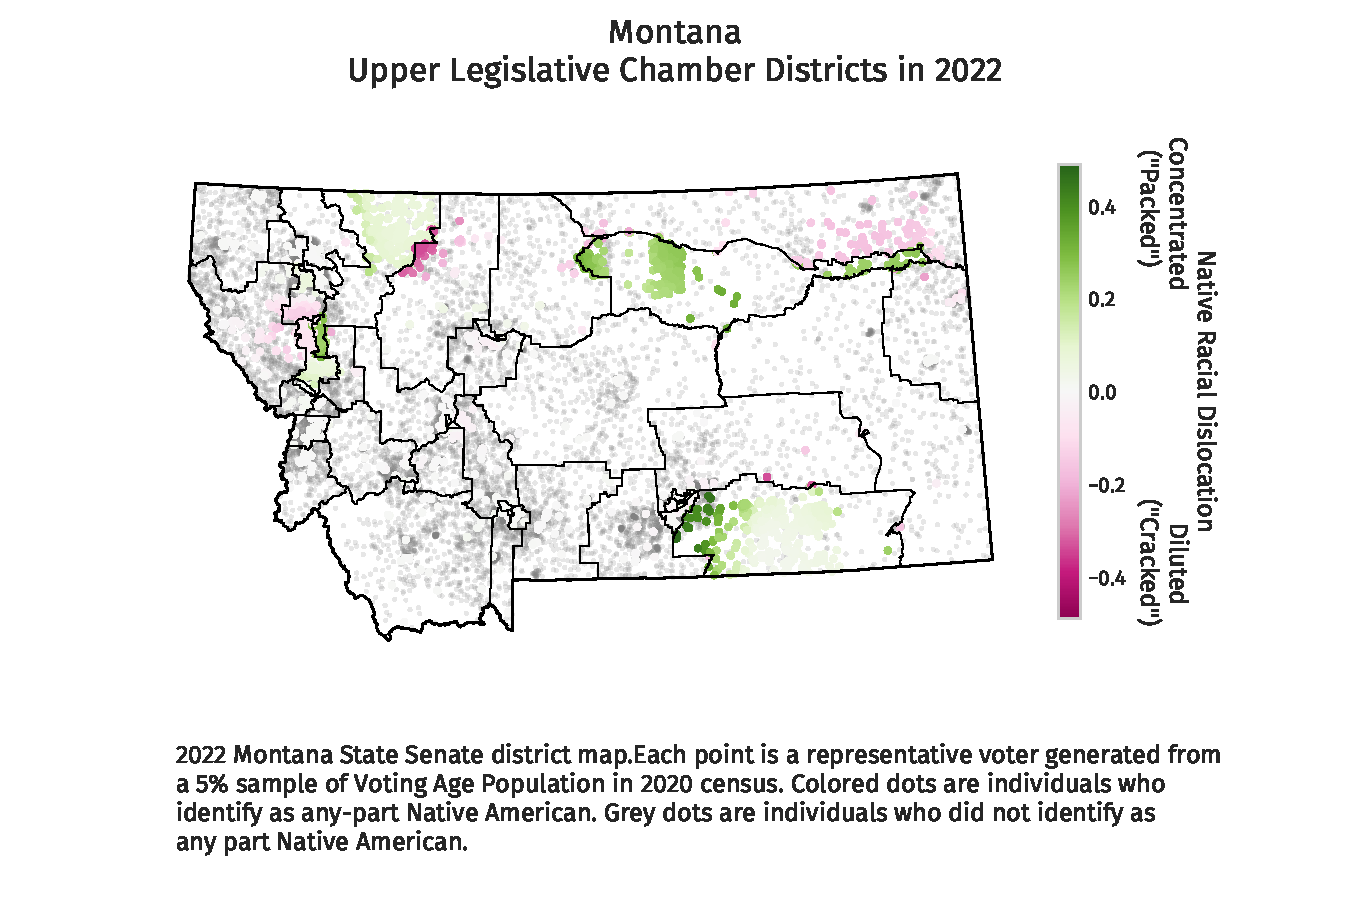
\includegraphics[trim={3cm 0 0 0}, clip,width=1.2\textwidth]{maps/MT_map2023_levelupper_MT_census2020_5pct.pdf} 
\caption{Montana Senate Dislocation Map (2022 Map)}
\label{fig:mt_map}
\end{figure}

% Check description below for completeness

Figure~\ref{fig:mt_map} is a map of Montana. The black lines on the map show the boundary of Montana's Senate Districts (``SD''s) from the 2022 redistricting cycle. Each dot on the map represents a single person who lived in Montana.  The total number of dots constitute a random sample of 5\% of Montana's population in 2020.

The dots differ between those in gray and those in color.  Each gray dot represents a non-Native person; each colored dot represents a Native-person. Non-Native persons are mapped to provide a representative view of where non-Native populations within the state reside; their dots are uniformly gray because we do not calculate dislocation values for them. The colored dots, representing Native persons, have colors that depend on their dislocation values. As shown on the color legend on the right, green indicates that the Native person is in a district with higher Native population than her similarly sized neighborhood (i.e. high positive values indicate packing), and pink indicates that the representative Native person is in a district with a lower Native population than her similarly sized neighborhood (i.e. high negative values indicate cracking).

Though the above figure is not of the highest resolution, the pdfs maps available on our online repository are. They are designed to both offer a birds-eye view of the state as a whole and to facilitate zooming in. Every district that is over 9\% NVAP is labeled.\footnote{This is, by nature, an arbitrary threshold. We chose it because it offers a buffer for evaluating districts that are or might soon be 25\% NVAP. Conventionally, to evaluate whether a district might satisfy prong 1 of \textit{Gingles} would be to determine whether a district could be majority Native (i.e. > 50\% Native VAP). The reason to look further down from the range around 50\% is that some state house representatives are elected at large from state Senate districts (e.g. Arizona, where two state house representatives are elected from each state Senate districts). Thus, in evaluating whether Section 2 might mandate the creation of a house district, 25\% (that is 50\% of 50\%) may be the relevant threshold. We display labels for all districts with over 18\% Native to maximize visibility of districts with significant NVAP.} The labels include the district identifier\footnote{HD for House Districts; SD for Senate Districts. Usually districts are identified by numbers, but Alaska uses letters of the alphabet and some states use a combination of both.} and the district's NVAP (AI is short for American Indian, the term the census bureau uses for Native race).

It is important to note all that these maps do not depict: the myriad other formally accepted redistricting criteria (e.g. respect for jurisdictional boundaries, compactness and preserving communities of interest\footnote{One important redistricting criteria that is especially relevant for Native populations might be the boundaries of tribes and tribal territories.}) and other political considerations (e.g. protecting incumbents) that no doubt influence linedrawers. These considerations are not visible in the maps presented; the goal is simply to evaluate the redistricting plans against the state's changing racial geography, not to offer a highly factually specific analysis of each individual district. That these maps do not contain any additional information about the states apart from their district boundaries and relative racial geography with respect to Native persons should only serve to highlight the unidimensional nature of these analyses; they are not meant to make definitive claims about the legitimacy of the enacted districting plans. Of course, other redistricting criteria, to the extent they can be mapped, could be added to these maps as additional layers for further investigation.

That we do not consider other redistricting criteria apart from racial geography makes clear that our use of the terms ``cracking'' and ``packing'' is meant to be purely descriptive.  District lines that descriptively pack or crack Native persons based only on the dislocation measure may not actually reflect \textit{legally actionable} cracking or packing. Implicit in any claim that our analyses demonstrate that the investigated maps are guilty of legally actionable cracking or packing is the idea that racial groups can constitute communities of interest that should be respected in the redistricting process.  But whether our analyses in fact tends to prove legally actionable cracking and packing depends on whether Native persons who live proximately to each other actually constitute a community of interest that should be respected in the redistricting process. A community of interest, as described in the redistricting literature, is infamously a nebulous and highly contextual concept; it is sometimes explicitly defined in racial terms and other times it has racial implications (for instance, individuals who rely on a particular geographic feature, for instance a river valley, for their economic and social activities). Thus, any allegation of \textit{legally actionable} packing and cracking cannot rely on Native dislocation analyses alone, as it is possible that Native persons who are concentrated or dispersed do not in fact all constitute the same community of interest. For instance, district lines that appear to crack Native communities by dividing them across two districts may in fact simply track county/city boundaries or geographic features (e.g. a ridge that divides two watersheds, which give rise to two historically distinctive communities). It is for these reasons that we do not make normative claims about any specific districts and instead draw our conclusions in the next section of the paper based on empirical regularities throughout the data.

\subsection{Dislocation results: tabulated}

Compiling dislocation measures across all study states and both levels of state legislative districts, we find that Native-majority districts do appear to be packed, in many cases, in an extreme manner.  This is true across districts in the previous redistricting cycle (maps first used in the 2018 elections and based on 2010 census data) and the current cycle (maps first used in the 2022 elections and based on 2020 census data). 

Most of these districts are a legacy of the Voting Rights Act.  Some are direct descendants of remedial districts drawn pursuant to Section 2 litigation, for instance HD 26A (South Dakota)\footnote{See \textit{Bone Shirt v. Hazeltine}, 461 F.3d 1011, 1023 (8th Cir. 2006).} and HDs 4, 5, 6, 9, 65, and 69 (New Mexico)\footnote{\cite{mccool2007native} at 83 (describing \textit{Jepsen v. Vigil-Giron}, a lawsuit brought by the Navajo and Jicarilla Apache Nations). For details about these districts, see Legislative Council Service, Redistricting Committee Final Report (Apr. 2002), File No. 208-01 at 101-03 (describing demographic composition of 2022 court ordered house district plan), available at \url{https://www.nmlegis.gov/Redistricting2011/Documents/02_REDISTRICTING\%20Report\%20FINAL\%20REPORT.pdf}}. Some were first drawn by legislatures with the understanding that they were required by Section 2, for instance HD 28A (South Dakota),\footnote{This majority-native house district, nested within Senate District 28 was created by the South Dakota Legislature in the 1990 round of redistricting “in order to protect minority voting rights.” \cite{mcdonald2007voting} at 208-09 ((describing and citing to Act to Redistrict the Legislature, ch.1, 1991 S.D. Sess. Laws 1st Spec. Sess. 1.).} many of the majority-Native districts in Alaska,\footnote{The 2000 redistricting board “clearly paid careful attention to the requirements of the VRA.” \cite{landreth2007voting} at 41-43. The two majority-Native senate districts and three majority-Native districts from the 2000 map cover the same geographies as subsequent and current majority-Native districts in Alaska, although the district labels have changed. To see visual maps from earlier redistricting plans in Alaska, \textit{see, e.g., id}. at 55 for 1994 Senate District Map.} and HD 33 (Wyoming).\footnote{Wyoming’s only majority-Native district was created in 1992 (and persists in similar form today). It is worth noting that until 1991, Wyoming’s state legislative districts were delineated by county lines. Re: Legal Research: Constitutional Apportionment of Legislators, Wyoming Legislative Service Office Memorandum (Sep. 10, 2025) at 2 (citing \textit{Gorin v. Karpan}, , 775 F. Supp. 1430 (D. Wyo. 1991), which struck down the county as district requirements of Article 3, Section 3 of the Wyoming Constitution on one-person, one-vote grounds), available at \url{https://wyoleg.gov/InterimCommittee/2025/S46-202509253-01LegalMemoConstitutionalRedistricting-September112025.pdf}. Though we could not find any firsthand accounts of the 1992 reapportionment, it is understood that HD 33, the only majority-Native state legislative district, was drawn to comply with Section 2 of the VRA. See Re: Principles of State Legislative Redistricting Law, Wyoming Legislative Service Office (May 26, 2021) at 5 (“In past redistricting cycles, the Wyoming Legislature has recognized that the Native American population residing within the Wind River Reservation in Fremont County constitutes a geographically distinct minority group with a sufficient population to warrant the creation of a Native American majority house district.”), available at \url{https://wyoleg.gov/Redistricting/Redistricting2020/RedistrictingMemorandum.pdf}; Cowboy State Daily, Four Candidates Vying to Win Wyoming’s Only American Indian Legislative District (Jun. 03, 2022) (describing HD33 as the “lone ‘majority-minority district’. . . which is a designation set by the U.S. Supreme Court in its 1986 interpretation of the Voting Rights Act and noting that HD33 “became a majority-minority district in 1992”), available at \url{https://cowboystatedaily.com/2022/06/03/four-candidates-vying-to-win-wyomings-only-american-indian-legislative-district/ }.} And though several other districts were not drawn specifically in response to Section 2 litigation, litigation may have played a persuasive role in the creation of these districts.  For instance, though the protracted litigation in the 1990 cycle over the failure to create a majority-Native district consisting of the Blackfeet and Flathead Indian Reservations in Montana did not result in a finding of legal liability under Section 2 of the Act, “[t]he 2000 [Redistricting] Commission chose to redistrict in a manner that had been proposed by the plaintiffs,” resulting in the creation of a new majority-Native district, SD 9.\footnote{Final Legislative Redistricting Plan based on the 2000 Census (Feb. 5, 2003) at 14-17, available at \url{https://archive.legmt.gov/content/committees/interim/2003_2004/dist_apport/work_plan/feb_04_finalplantosos.pdf}.} Finally, several of these districts were first created under pressure from the Department of Justice through the pre-clearance process pursuant to Section 5 of the Voting Rights Act, which is governed by a similar but not identical legal standard to what Section 2 requires. These include many of the majority-Native districts in Alaska,\footnote{The Alaska legislature redrew its maps after the Department of Justice objected to house and senate districts from the 1990 cycle; many of the majority-Native districts from this map resemble current majority-Native districts. \textit{See} \cite{landreth2007voting} at 41-43; DOJ Objection Letter to Alaska (Sep. 28, 1993), available at \url{https://www.justice.gov/crt/voting-determination-letters-alaska}.} Arizona,\footnote{Similar to Alaska, the Department of Justice formally objected to Arizona’s 1982 redistricting plan over dilution of Native votes from the San Carlos Indian Reservation.  DOJ Objection Letter to Arizona (Mar. 8, 1982) available at \url{http://www.justice.gov/crt/records/vot/obj_letters/letters/AZ/AZ-1040.pdf}. The DOJ also objected to the 2002 maps, but primarily on the ground of retrogression of Hispanic voting strength. DOJ Objection Letter to Arizona (May 20, 2022), available at \url{https://www.justice.gov/sites/default/files/crt/legacy/2014/05/30/l_020520.pdf}.} and SD 28 (South Dakota).\footnote{Unlike Alaska and Arizona, the pressure exerted from the Department of Justice on South Dakota was less formal; no formal objection was ever made.  But more informally, the Department (combined with pressure from the Civil Rights Commission as well) influenced the creation of SD 28 in the 1980 redistricting cycle. \textit{See Bone Shirt v. Hazeltine}, 336 F. Supp. 2d 976, 981 (D.S.D. 2004) (describing the creation of the first majority-Native district in South Dakota “[a]fter the national Civil Rights Commission received the state commission's report, the Department of Justice instructed South Dakota that it would not approve its reapportionment plan unless the state created a substantially Indian district.”)}

Figure~\ref{fig:Dislocation_Box} presents dislocation scores separately for each redistricting cycle. The first subplot compiles the dislocation scores from the 2018 maps and plots their values based on the percentage Native of the district that they reside in, while the second subplot shows results for the 2022 districting cycle.

\begin{figure}[h]
  \centering
  
\includegraphics[width=0.45\textwidth]{figures/dislocation_by_district_AI_map2018_census2010_chamberall.png} 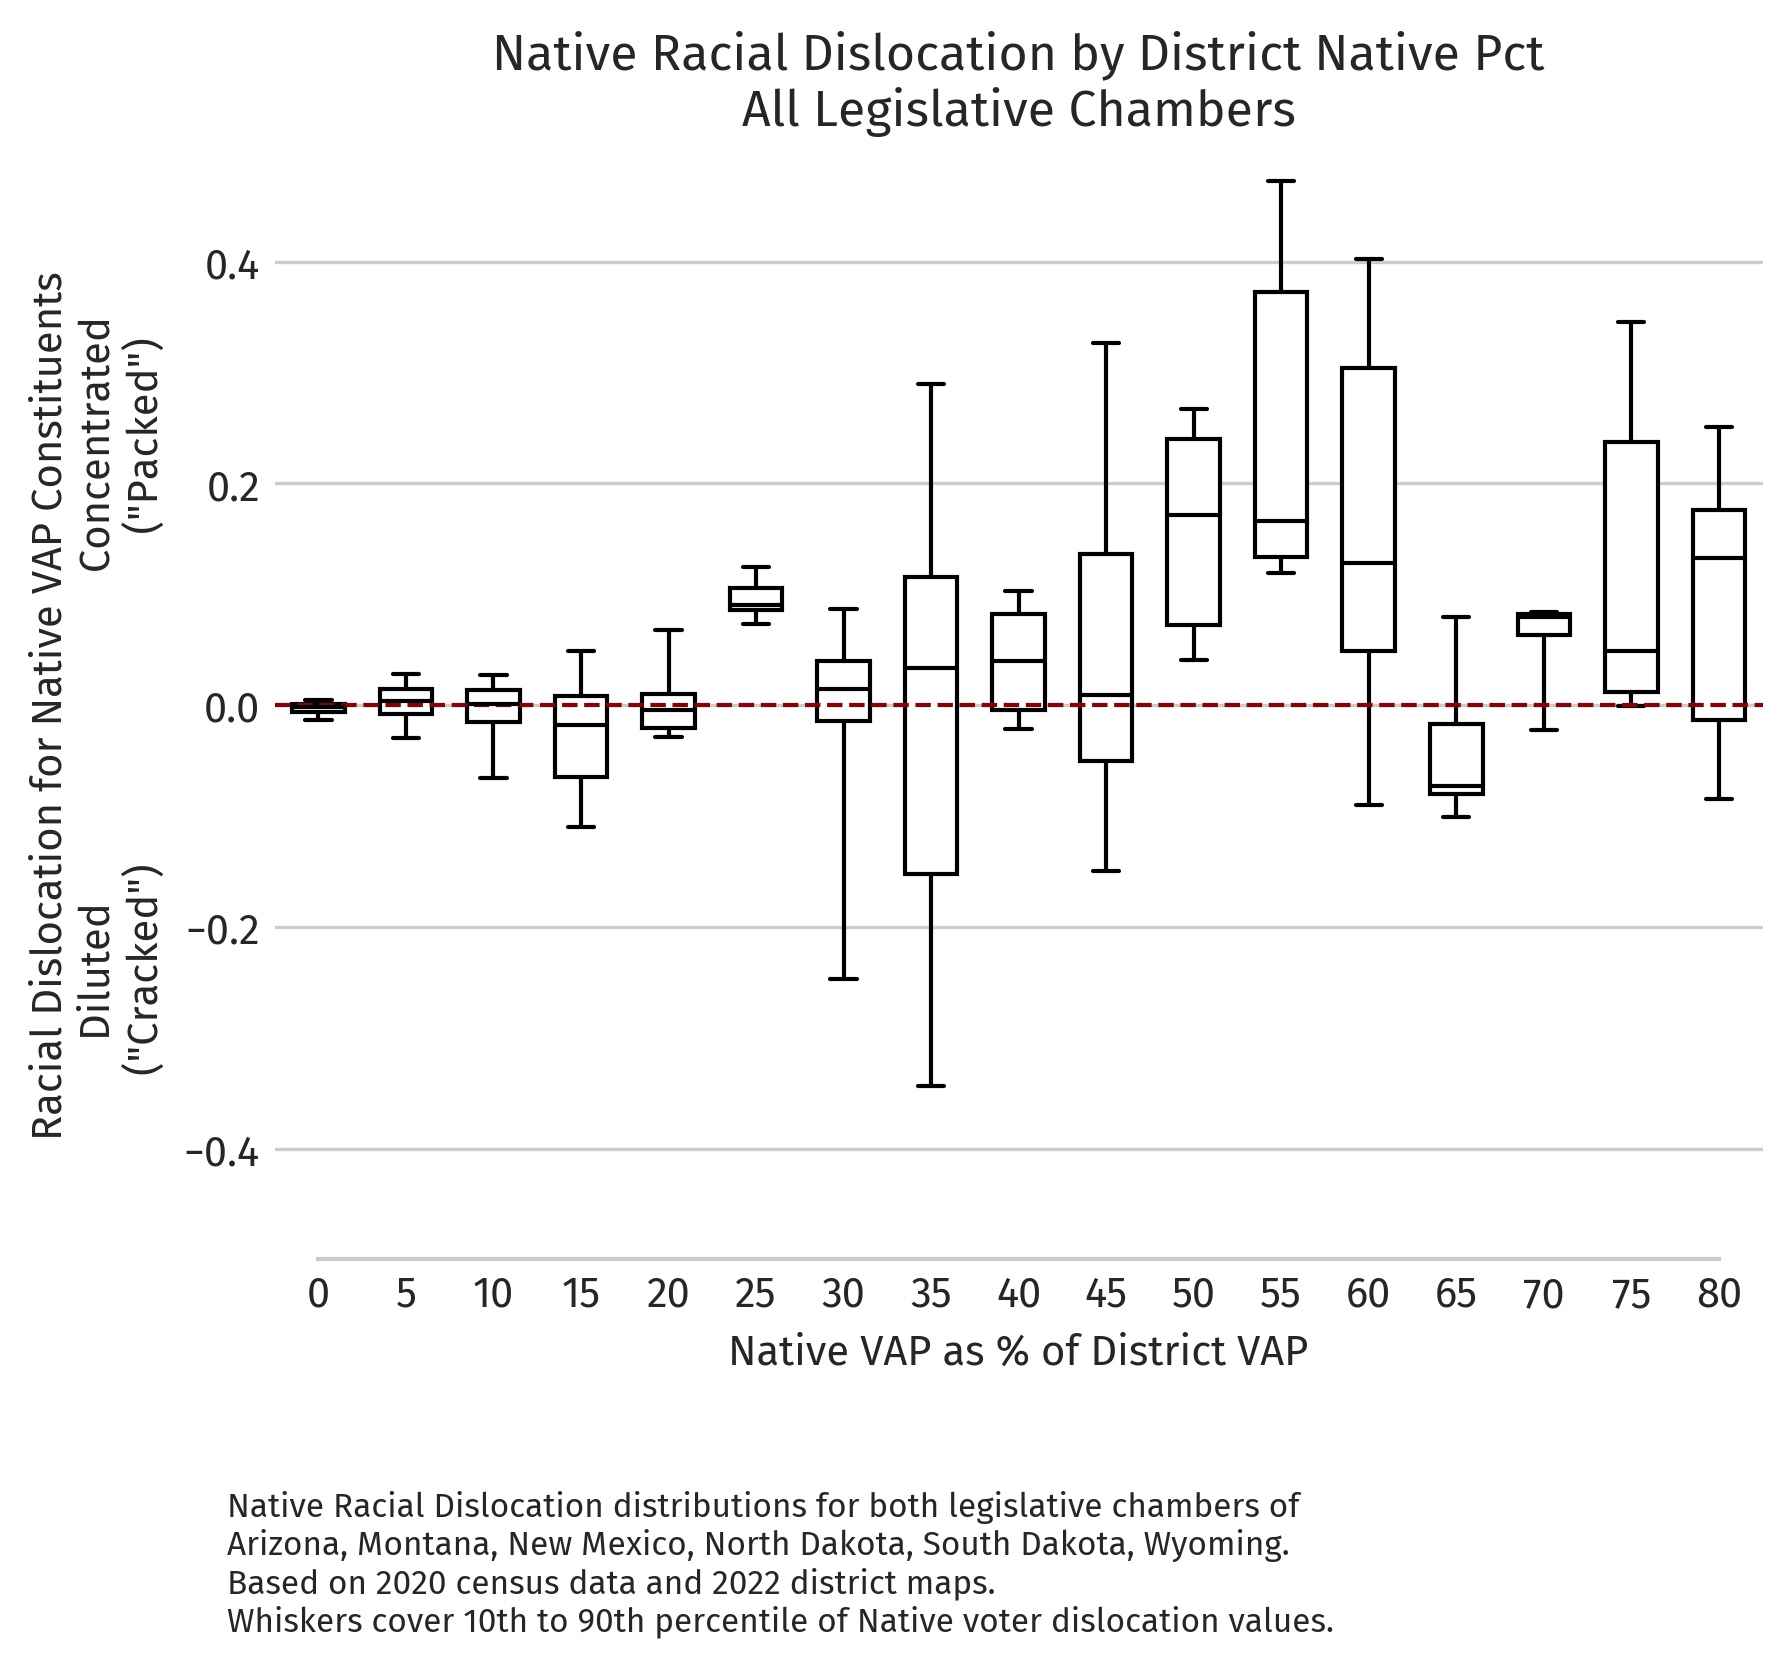
\includegraphics[width=0.45\textwidth]{figures/dislocation_by_district_AI_map2023_census2020_chamberall.png}
  \caption{Dislocation by District NVAP (2018 and 2022 districts)}
  \label{fig:Dislocation_Box}
\end{figure}

The x-axis sorts the values by ascending order of Native VAP in the districts.  The y-axis presents the dislocation values across these types of districts.  It is centered on 0 (where the district's Native composition is the same as the immediate neighborhood of the same size).  Recall that high positive values suggest packing (one's district has more Native persons than one's neighborhood of the same size) and high negative values suggest cracking (one's district has fewer Native persons than one's neighborhood of the same size). Dislocation scores are displayed in the form of boxes plots to show the full range of dislocation values in these differently constituted districts: the line in the middle of the box shows the median dislocation value (i.e. the 50th percentile), the top and bottom of the box the 75th and 25th percentiles, and the top and bottom arms (or whiskers) the 10th and 90th percentile values.

Focusing first on the majority-Native districts across both the 2012 and 2022 redistricting cycles, the figures confirm that there is significant packing in these districts.  Dislocation values for districts with Native VAP percentages above 50\% almost universally skew positive.  And the magnitude of positive values can be quite high.  For instance, among districts in both the 2012 and 2022 redistricting cycles comprising between 75-80\% NVAP, there was, on average, 10 percentage points more Native persons than in their immediate neighborhood of a comparable size.  And across both redistricting cycles, there are at least a small handful of districts with extremely high dislocation scores exceeding a 40 percentage point difference between the district's Native percentage and that of the immediate neighborhood.  Though this finding is not necessarily surprising given the very high Native VAP districts that were observed from Figure~\ref{fig:Bar_NVAP_ElectNR} and Figure~\ref{fig:Bar_NVAP_ElectNR_bystate} earlier in the paper, the dislocation measures provide validation for our observation as they allow us to reject the hypothesis that racial geography is responsible for the composition of these districts.  The dislocation measures also provide precise estimates that describe the extent of packing in these districts.  The dislocation measures also show that the concern over packing is not necessarily most acute for districts with highest Native percentages.  Indeed, it is districts between the 55-65\% Native VAP range that exhibit some of the most extreme instances of packing.

More unexpectedly, Figure~\ref{fig:Dislocation_Box} shed light on some limited but not insignificant cracking in districts in which Native persons do not constitute a majority.  For instance, some districts with between 45-50\% Native VAP (and to a lesser extent districts with 35-40\% and 40-45\% VAP as well) are quite severely cracked.

Finally, we observe little evidence of significant packing or cracking in districts with few Native voters (under 20\% Native VAP).

\subsection{Packing in Majority-Native districts}

Why do we observe widespread packing in Native-majority districts and some cracking in non-Native-majority districts---while Section 2 is operative?  The answer is that though Section 2 intervenes in important ways to combat vote dilution, it does so only when certain conditions are met.  Much of the kind of dilution we observe here is likely not actionable under Section 2 in large part because of the first precondition of \textit{Gingles}.  It is certainly possible for a majority-Native district to violate Section 2.  But that does not occur unless and until the first \textit{Gingles} condition is met: that the minority population is large enough to constitute a majority in a district.  For this condition to be triggered to address packing in a majority-Native district, it means that a second majority-Native district can be drawn in its vicinity.  Similarly, it is likely that the cracking we observe is in districts and areas in which the Native population is not large enough to meet the first \textit{Gingles} condition.  Given the numerical disadvantage that Native communities are in, even in the study states, that threshold is very hard to meet.  Even in the face of significant higher rates of population growth in the Native versus non-Native populations, the threshold imposed by the first \textit{Gingles} condition is one that is very hard to meet given that the Native population is significantly outnumbered by the non-Native population.   

Though the instances of packing do not trigger Section 2 liability, they do have substantive consequences for Native populations in those districts and their vicinity.  In particular, these districts can nevertheless deprive Native communities of the opportunity to \textit{influence} politics and policy-making, even if it might not deprive them of the opportunity to \textit{elect} their candidates of choice. Imagine two different scenarios: first, an 80\% NVAP district next to a 10\% NVAP district, or second, a 60\% Native district next to a 30\% NVAP district. Imagine further that the first precondition of \textit{Gingles} is not met in either case: there are not enough Native persons in this area to draw a second Native-majority district. Though these two scenarios are equal from the perspective of Section 2 (in that neither violate the Act), they are not equal in terms of minority opportunity to influence elections.  While Native persons can only elect one Native candidate-of-choice from both districts in both scenarios, they have much more influence over who is elected overall in the second scenario. (For instance, they may constitute a majority of voters in the primary election and thus heavily influence who the elected representative is. \textit{See }\cite{katz2004resurrecting}.) 

Section 2 leaves state legislatures and other linedrawers free to choose between the two scenarios.  Though it is possible that they would choose the latter, there is no legal obligation (or litigation pressure) on them to do so. Our evidence shows that, in the absence of such a legal obligation, they have indeed elected not to draw districts in a way that enhances Native influence.\footnote{This is perhaps unsurprising given the historical intransigence of state legislatures to drawn Native opportunity districts that are mandated by Section 2. \cite{mcdonald2010american}} 

To make concrete these observations, that enabling minority opportunity-to-elect through the creation of majority-Native districts may in fact diminish minority ability-to-influence, we present two districts from Montana as examples.  Consider, first, the example of Montana Senate District (``SD'') 16 from the 2022 redistricting cycle, who, along with its neighbors are shown in Figure~\ref{fig:MT_SD16}:

\begin{figure}[h]
  \centering
  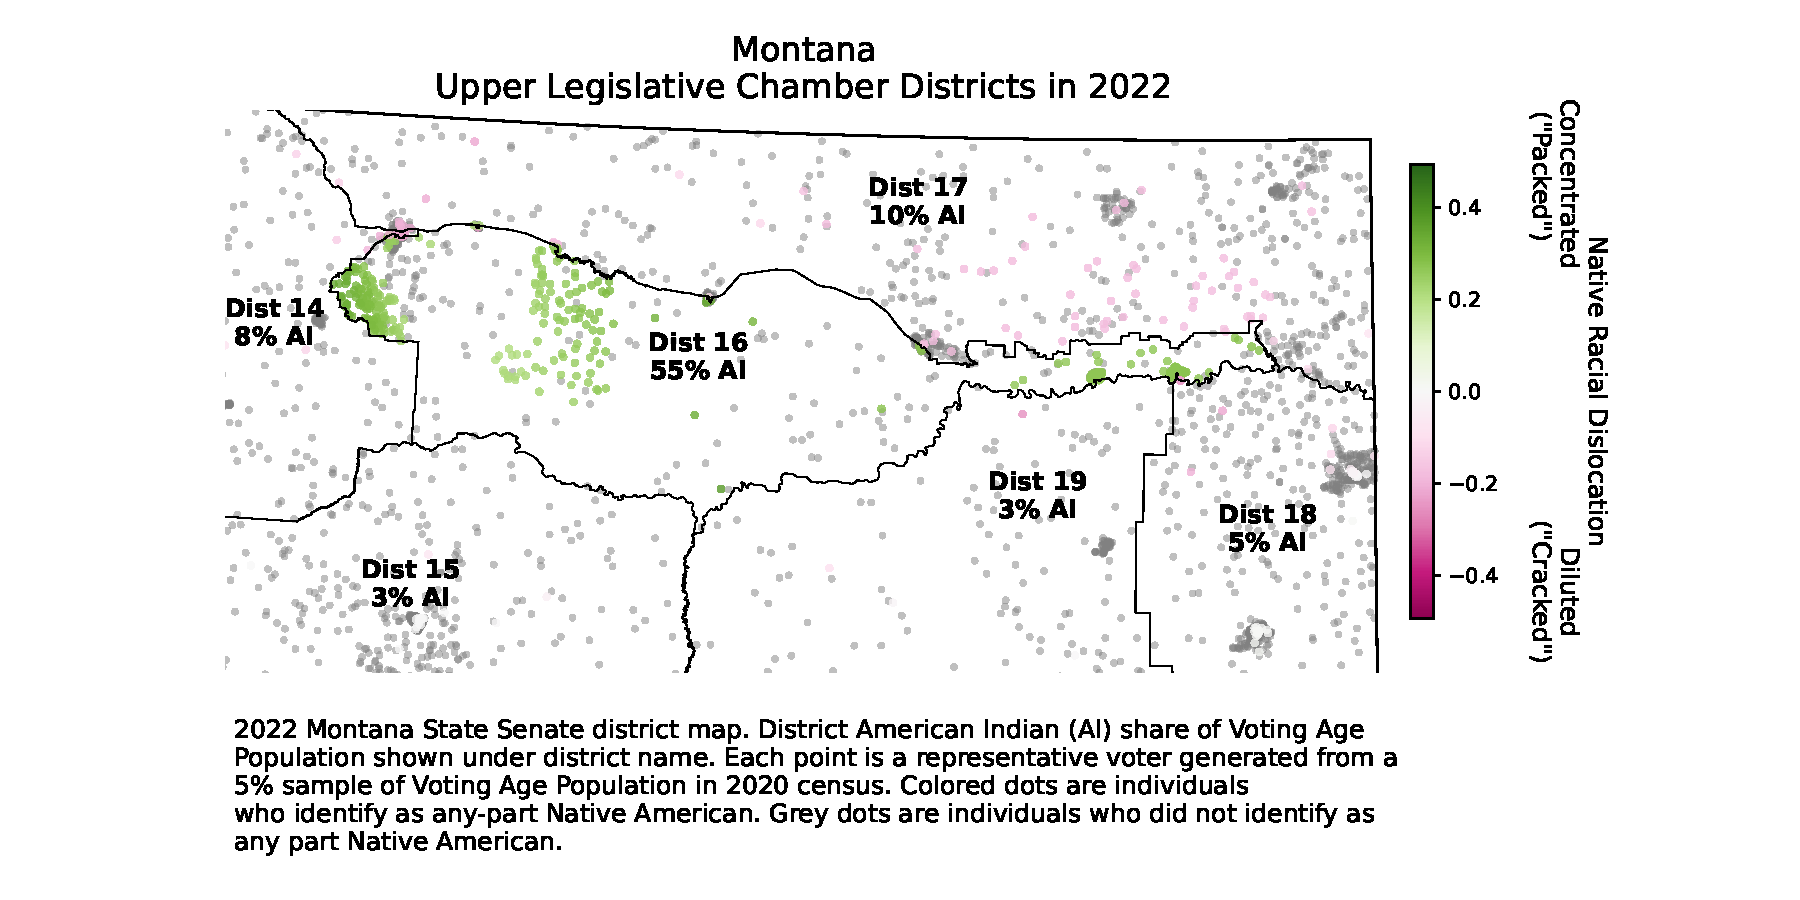
\includegraphics[trim={3cm 0 0 0}, clip,width=1.2\textwidth]{maps/MT_upper16_specific_map2023_MT_census2020_5pct.pdf}
  \caption{Montana SD 16 (2022 districts)}
  \label{fig:MT_SD16}
\end{figure}

The focus of Figure~\ref{fig:MT_SD16} is Montana's SD 16, which is a majority-Native district (59\% NVAP).  Recall that each dot represents a person: gray dots depict non-Native individuals, and colored dots (along the spectrum provided on the right) depict Native individuals.  Consistent with what we describe in earlier paragraphs, SD 16 includes many Native persons who are packed (as indicated by the high positive dislocation values in green).  Vitally, in both corners of SD 16, it is surrounded, in neighboring districts, by Native persons who are cracked in those districts.  Yet, because the number of Native persons who are packed in SD 16 and those who are cracked in SDs 14 and 17 (and to a lesser extent in SDs 15 and 18) are insufficient to result in a second majority-Native district in this area, the dilution of influence of Native persons is tolerated by Section 2.

A similar dynamic exists for the house districts in this same region of Montana.  Next, we present House Districts (``HD''s) 31 and 32 in Montana, which are two districts nested\footnote{Nesting is a redistricting practice of drawing two house districts within one senate district, a not uncommon practice in state legislative redistricting more generally and among our study states. A recent article on nesting claims that eight states currently have two single-member House/Assembly districts nested in each Senate district. \cite{caldera2020mathematics}. Another source, Ballotpedia, claims that a total of 18 does so. \textit{See}, Nesting, Ballotpedia, available at: \url{https://ballotpedia.org/Nesting}. Yet another source, All About Redistricting, claims that a total of 17 does so, see \url{https://redistricting.lls.edu/redistricting-101/where-are-the-lines-drawn/criteria-for-state-legislative-districts/}. We independently determined that among our study states, nesting is practiced in Alaska, North Dakota, Montana, South Dakota, and Wyoming. In this paper, we take this practice for granted while also noting that it is not uncontroversial even if it is widespread, and that scholarly attention to the practice has been sparse. \textit{But see }\cite{caldera2020mathematics,cain2007implications}.} within SD 16, in Figure~\ref{fig:MT_HD3132}:

\begin{figure}[h]
  \centering
  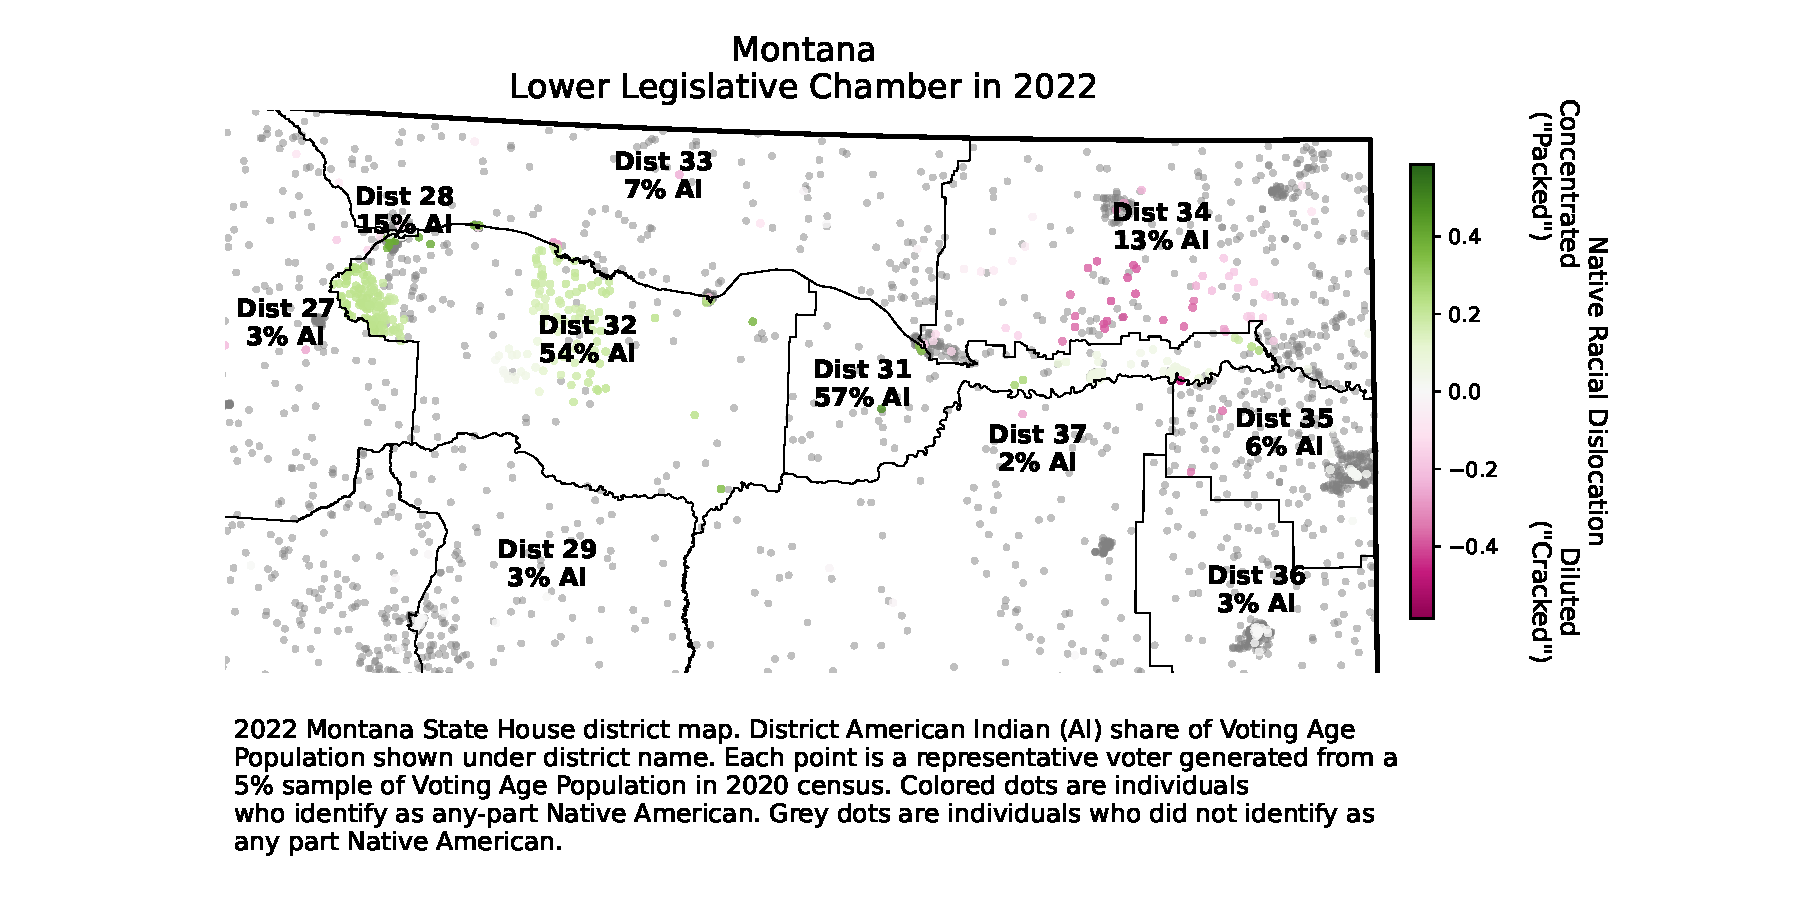
\includegraphics[width=0.8\textwidth]{maps/MT_lower31_specific_map2023_MT_census2020_5pct.pdf}
  \caption{Montana HDs 31 \& 32 (2022 districts)}
  \label{fig:MT_HD3132}
\end{figure}

HDs 31 and 32 are both Native-majority districts.  Consistent with our observation earlier, the extent of cracking in these districts does not map on simply to the Native VAP percentages in the districts: HD 32, though it has a smaller Native VAP percentage, has Native constituents who are more packed than those in HD 31. And though the persons who are packed in HDs 31 and 32 are similar to those who were packed in SD 16, the severity of cracking in neighboring districts is different than that produced by the senate districts in Figure~\ref{fig:MT_SD16}.  This is consistent with findings in the literature that vote dilution can and often varies between levels of districting.\footnote{\cite{eubank_rodden_2020}}  But the dynamic that we observed in the senate districts, that a majority-Native district can nevertheless produce dilution of Native influence in neighboring districts without running afoul of Section 2, is also present here. In Figure~\ref{fig:MT_HD3132}, that dynamic is most extreme between HD 31 and HD 34: Native individuals along the arm of HD 31, a Native-majority district, are lightly packed, and Native individuals across the border in HD 34 (with 14\% NVAP) are quite severely cracked.  Once again, what is critical about these observations is that these vote dilution effects are consistent with the application of Section 2 because a second Native-majority district cannot be drawn here.\footnote{This is not to say that these conditions cannot be met.  Indeed, they have been met in extreme cases. \textit{Bone Shirt v. Hazeltine}, 461 F.3d 1011 (8th Cir. 2006), involved a Section 2 challenge to Senate District 27, “with a ninety percent Native-American population,” which neighbored Senate District 26, with “thirty percent Native-American population.” \textit{Id}. at 1016.  Plaintiffs produced a proposed remedial map that reduced the Native population in District 27 (but was still a Native-majority district) and created a new majority-Native house district in the vicinity of Senate District 26 that was majority-Native. \textit{Id}. at 1018-19. On this basis, the Court of Appeals affirmed the district court's finding of a Section 2 violation under Gingles I. \textit{Id}.}

Our empirical results strength an important and longstanding critique of Section 2, fleshed out by Lani Guinier in three pivotal articles,\footnote{\cite{guinier1989keeping,guinier1991seats,guinier1991triumph}, \textit{see also \cite{karlan1995tyranny}}} that it focuses on minority voters' ability to elect candidates of success and overlooks their ability to exert political influence. Though this critique goes deeper than the issues we investigate in this paper (for instance on the ability of minority groups to achieve substantive political outcomes and command legislative influence), our findings provide empirical support for the critique.  Indeed, we show that majority-Native districts may not only provide ``token'' representation to Native individuals, but in fact serve as a fig-leaf for diluting the influence of Native voters through packing.  To the extent that racial geography would be posited as an explanation or excuse for these ultra-safe Native districts, our findings suggest it is not valid, at least with respect to many of such districts.

If not racial geography, what accounts for these districts?  After observing the prevalence of safe majority-Black districts in earlier decades, \cite{pildes2007decline} noted that political factors may account for why safe districts became the norm.  As concern mounted in more recent decades about partisan gerrymandering, scholars started to voice concerns over the use of safe districts to enhance partisan interests. \cite{pildes2001voting,issacharoff2002gerrymandering}. The theory for such a dynamic depends on an important factual assumption: that minority voters tend to support Democratic candidates.\footnote{The phenomenon that race and party have become more and more intertwined over time has been described as conjoined polarization. \cite{cain2016blurred}.}  If so, then a district drawn to safely elect minority candidates of choice will also be reliably safe Democratic districts.  If we make additional assumptions about residential patterns, for instance, that minority voters tend to live much closer to white Democrats than white Republicans, then majority-minority districts drawn in the area will not only be safe Democratic districts, but packed Democratic districts.

It is clear that whether and where such a dynamic exists, and how strong it is, is an empirical question that depends on a variety of important factual predicates: the size of the minority population, how strong their alignment with a party is, whether they live close to white voters who share their party preferences, and the size of the districts drawn.  The relationship between race-motivated districting and partisan gerrymandering has always been a complex one, and arguments about whether race-motivated districting produces partisan outcomes have been used instrumentally, for instance, to undermine Section 2. \textit{See, e.g.}, \cite{karlan1997loss} (critiquing the ``bleaching hypothesis'' that the creation of majority-black districts injure Black voters by reducing their influence in neighboring, more conservative districts). And there are reasons to believe that Section 2's requirements do not generally inure to the benefit of the Republican Party. \textit{See} \cite{cox2011reconsidering}.

But it is also clear that when certain factual conditions exist in discrete places and districts, safe Section 2 districts could produce partisan advantages. \footnote{Certainly as a historical matter, when there was an absence of a legal mandate to create minority opportunity-to-elect districts, there are many instances in which drawing majority-minority districts was a useful strategy to enhance partisan interests.  \textit{See} \cite{crum2024riddle}.} A important indication that Section 2 compliance is a smokescreen for partisan gerrymandering is how compliance with Section 2 is accomplished. What Section 2 actually demands is a searching factual inquiry into the conditions that would allow for minority voters to elect their candidates-of-choice; attempts to invoke it as a smokescreen would instead rely on simplistic racial targets.  \cite{levitt2015quick}.  Several such examples are present in racial gerrymandering cases that the Supreme Court heard relating to maps drawn in the 2012 redistricting cycle.\footnote{\textit{See} \cite{crum2024riddle} for context on how these second wave \textit{Shaw} cases fit into the broader doctrine.}  Alabama, for instance, claimed that it had sought to comply with Section 2 when it drew its 2012 maps by ``maintain[ing] existing racial percentages'' from the previous decade's maps.\footnote{\textit{Alabama Legislative Black Caucus v. Alabama}, 575 U.S. 254, 273 (2015).} (The Supreme Court clarified, in \textit{Alabama Legislative Black Caucus v. Alabama}, that the VRA did not require Alabama to ``maintain a particular numerical minority percentage,'' but rather, to ``maintain a minority's ability to elect a preferred candidate of choice.''\footnote{\textit{Id}. at 275. Though it was technically Section 5 of the VRA that the Court was interpreting, the same is true of Section 2.} Similarly, in \textit{Cooper v. Harris},\footnote{581 U.S. 285 (2017).} the North Carolina legislature similarly established improper ``racial targets'' in two congressional districts.

Implicit in these cases is that adopting the simplistic (or cartoonish, \cite{levitt2015quick}) interpretation of Section 2 as establishing mechanical racial targets advances partisan goals. \cite{hasen2015racial,hasen2016election,hasen2017race,levitt2017race,stephanopoulos2017walking}.  What is clear with respect to the ultra-safe Native-majority districts we observe is that they \textit{could} be a product of partisan intentions, just as the implicated districts in \textit{ALBC} and \textit{Cooper} were.  Indeed, our analyses make clear that racial geography does not explain these districts.  But our analyses do not allow us to make direct conclusions about whether partisan motivations do.  Once again, it would be imprudent to assume that dynamics that may have been true for other racial minorities in other contexts apply to Native-majority districts.  For one, Native voters may not be as closely aligned with a single political party.  And their residential patterns may not be similar to other racial minorities.  A complete understanding of the dynamics that produce ultra-safe Native districts will require further work to investigate the presence and strength of political and other motivations.

\section{Conclusion}

In this paper, we have shown three things about the relationship between Native representation and Section 2.  First, Section 2 is not (and was never) the exclusive driver of Native representation.  Many Native representatives are and have been elected from states and districts in which Section 2 is or was not, in fact, operational.  Second, Section 2 remains an important driver of Native representation in the study states (primarily Mountain West states with significant Native population and a history of Section 2 litigation), although even in these states, \textit{proportionally} more Native representatives are elected from non-Native-majority districts.  Third, in the study states, Section 2 does not address certain vote dilution threats to Native representation.  More specifically, that threat is presented primarily in the form of packing in majority-Native districts (who owe their existence to Section 2).

Regardless of whether Section 2 remains, our findings have important implications.  If Section 2 needs to be replaced, at the federal or state levels, its replacement should be attune to not only what Section 2 accomplished but also what it did not.  And if it survives, the vote dilution consequences observed under the Act should at least be known and investigated.

A key finding from this paper is how much vote dilution can occur for a minority population that is not addressed by Section 2.  Because of the extreme numerical minority status of Native persons in the study states, Section 2 is unlikely to support the creation of additional Native-influence, not to mention Native-opportunity-to-elect, districts for a while to come.  Indeed, even in the presence of significant population growth, Section 2's protections would not apply simply because the total size of the Native population is relatively small within the state.  Without a legal mandate for the creation of influence districts, Native persons may see many of their votes wasted, either through concentration in already bloated Native-majority districts or dispersed in small numbers across several districts.

 Though the legal requirements of Section 2 apply uniformly across racial minorities, because racial minorities are not all similarly situated, a requirement like the first \textit{Gingles} precondition may affect different racial minorities differently.  Put more simply, the vote dilution that we find is the result not of disparate treatment under Section 2, but of disparate impact.  The Guinier critique that Section 2 privileges ability-to-elect at the expense of influence hits especially hard in this context.

 If Section 2 is struck down or significantly narrowed, it will be state Voting Rights Acts that will have to address vote dilution locally.  It is the case that most existing state VRAs already abandon \textit{Gingles}'s first prong \cite{greenwood_stephanopoulos_2023}, likely because it is already considered an onerous requirement:
\cite{greenwood_stephanopoulos_2023} describe it as ``often the highest hurdle for plaintiffs under Section 2''. Our paper provides an additional reason based on distributive justice for the ``renunciation''\cite{greenwood_stephanopoulos_2023} of the first \textit{Gingles} condition: it imposes disparate burdens on racial minorities.  Indeed, the hurdle is highest for racial minorities with the smallest populations. To the extent that racial minorities that are an extreme numerical minority are especially in need of remedial statutes like state VRAs to enjoy full and equal political opportunities, or that political influence may be especially meaningful for these groups, our findings provide an independent reason for reconsidering the first \textit{Gingles} precondition.

Another key consideration in designing Section 2's replacement, if desired, is sensitivity to the underlying racial geography of the relevant state.  As our results show, the percentage of Native VAP in a district does not automatically signal vote dilution.  Though we generally observed packing in districts with high Native VAP, the relationship between the two was not linear: surprisingly, districts with very high Native VAP percentages were less packed than districts with less.  Institutional design choices, like the first condition of \textit{Gingles}, can produce disparate outcomes depending on the underlying racial geography.

A loss of Section 2 should prompt voting rights scholars to address existing critiques and think creatively and in a nuanced fashion about the right institutional solutions to address vote dilution where it exists. There has been nothing short of revolutionary change in the study of redistricting in the last decade thanks to methodological innovations in detecting and measuring partisan gerrymanders.  Among these changes is an understanding of the highly contextual role that political geography plays in the fairness of districting outcomes.  That understanding should inform future reform efforts of districting processes and outcomes, not just those relating to partisan gerrymandering.  Our findings make clear that efforts to revive or re-produce Section 2 should be guided by nuanced and contextual analysis of effects on all relevant racial minorities.  Many have persuasively argued that any replacement for Section 2 (and the Voting Rights Act more generally) should adopt a different approach.  \textit{See, e.g., }\cite{charles2014voting,charles2017race,charles2018slouching,pildes2000diffusion}. This paper does not take a position on which of these approaches is the most feasible or desirable.  But it does warn that there are strong reasons to anticipate that even neutral, generally-applicable rules and standards may have multifarious effects depending on the racial minority group and depending on the level of districting.  These effects should be investigated and understood before or when potentially long-lasting legal and design choices are made.











%------------------------------------------------ REFERENCES -------------------------------------------------%
\singlespacing
\clearpage
\newpage


\bibliography{references.bib}
\bibliographystyle{apsr.bst}

\newpage
\appendix

\section{Native Representation Probabilities, 2012-2020 Districting Cycle}\label{app:elect_probability_2010}

Figure~\ref{fig:Plot_NRProb2010} below plots the relationship between whether a district has, at any point, elected a Native representative during the 2012-2020 districting cycle. Districts from the end of the districting cycle (2018) are used to ensure only legally compliant districts are considered. District demographic data comes from the 2010 census.

\begin{figure}[h]
  \centering
  \includegraphics[width=0.8\textwidth]{figures/native_reps_probability_plot_census2010.png}
  \caption{Native VAP \& Probability of Electing Native Representatives (2010)}
  \label{fig:Plot_NRProb2010}
\end{figure}


\section{Dislocation results: proportional instead of absolute dislocation}
In this subsection, we present analogous analyses to those presented in Figure~\ref{fig:Dislocation_Box} using proportional, instead of absolute, dislocation values. Though we think that absolute dislocation values are more intuitive and thus present those results in the main paper, studies of partisan gerrymandering have conventionally analyzed proportional dislocation values. Thus, we supplement our paper with proportional dislocation values as well.

First, we present the proportional dislocation values for the 2012 districts (analogous to Figure~\ref{fig:Dislocation_Box}):
\begin{figure}[h]
  \centering
  \includegraphics[width=0.8\textwidth]{figures/proportinal_dislocation_by_district_AI_map2018_census2010_chamberall.png}
  \caption{Proportional Dislocation by District NVAP (2012 districts)}
  \label{fig:Prop_Dislocation_Box_2010}
\end{figure}

Next, we present the proportional dislocation values for the 2020 districts:
\begin{figure}[h]
  \centering
  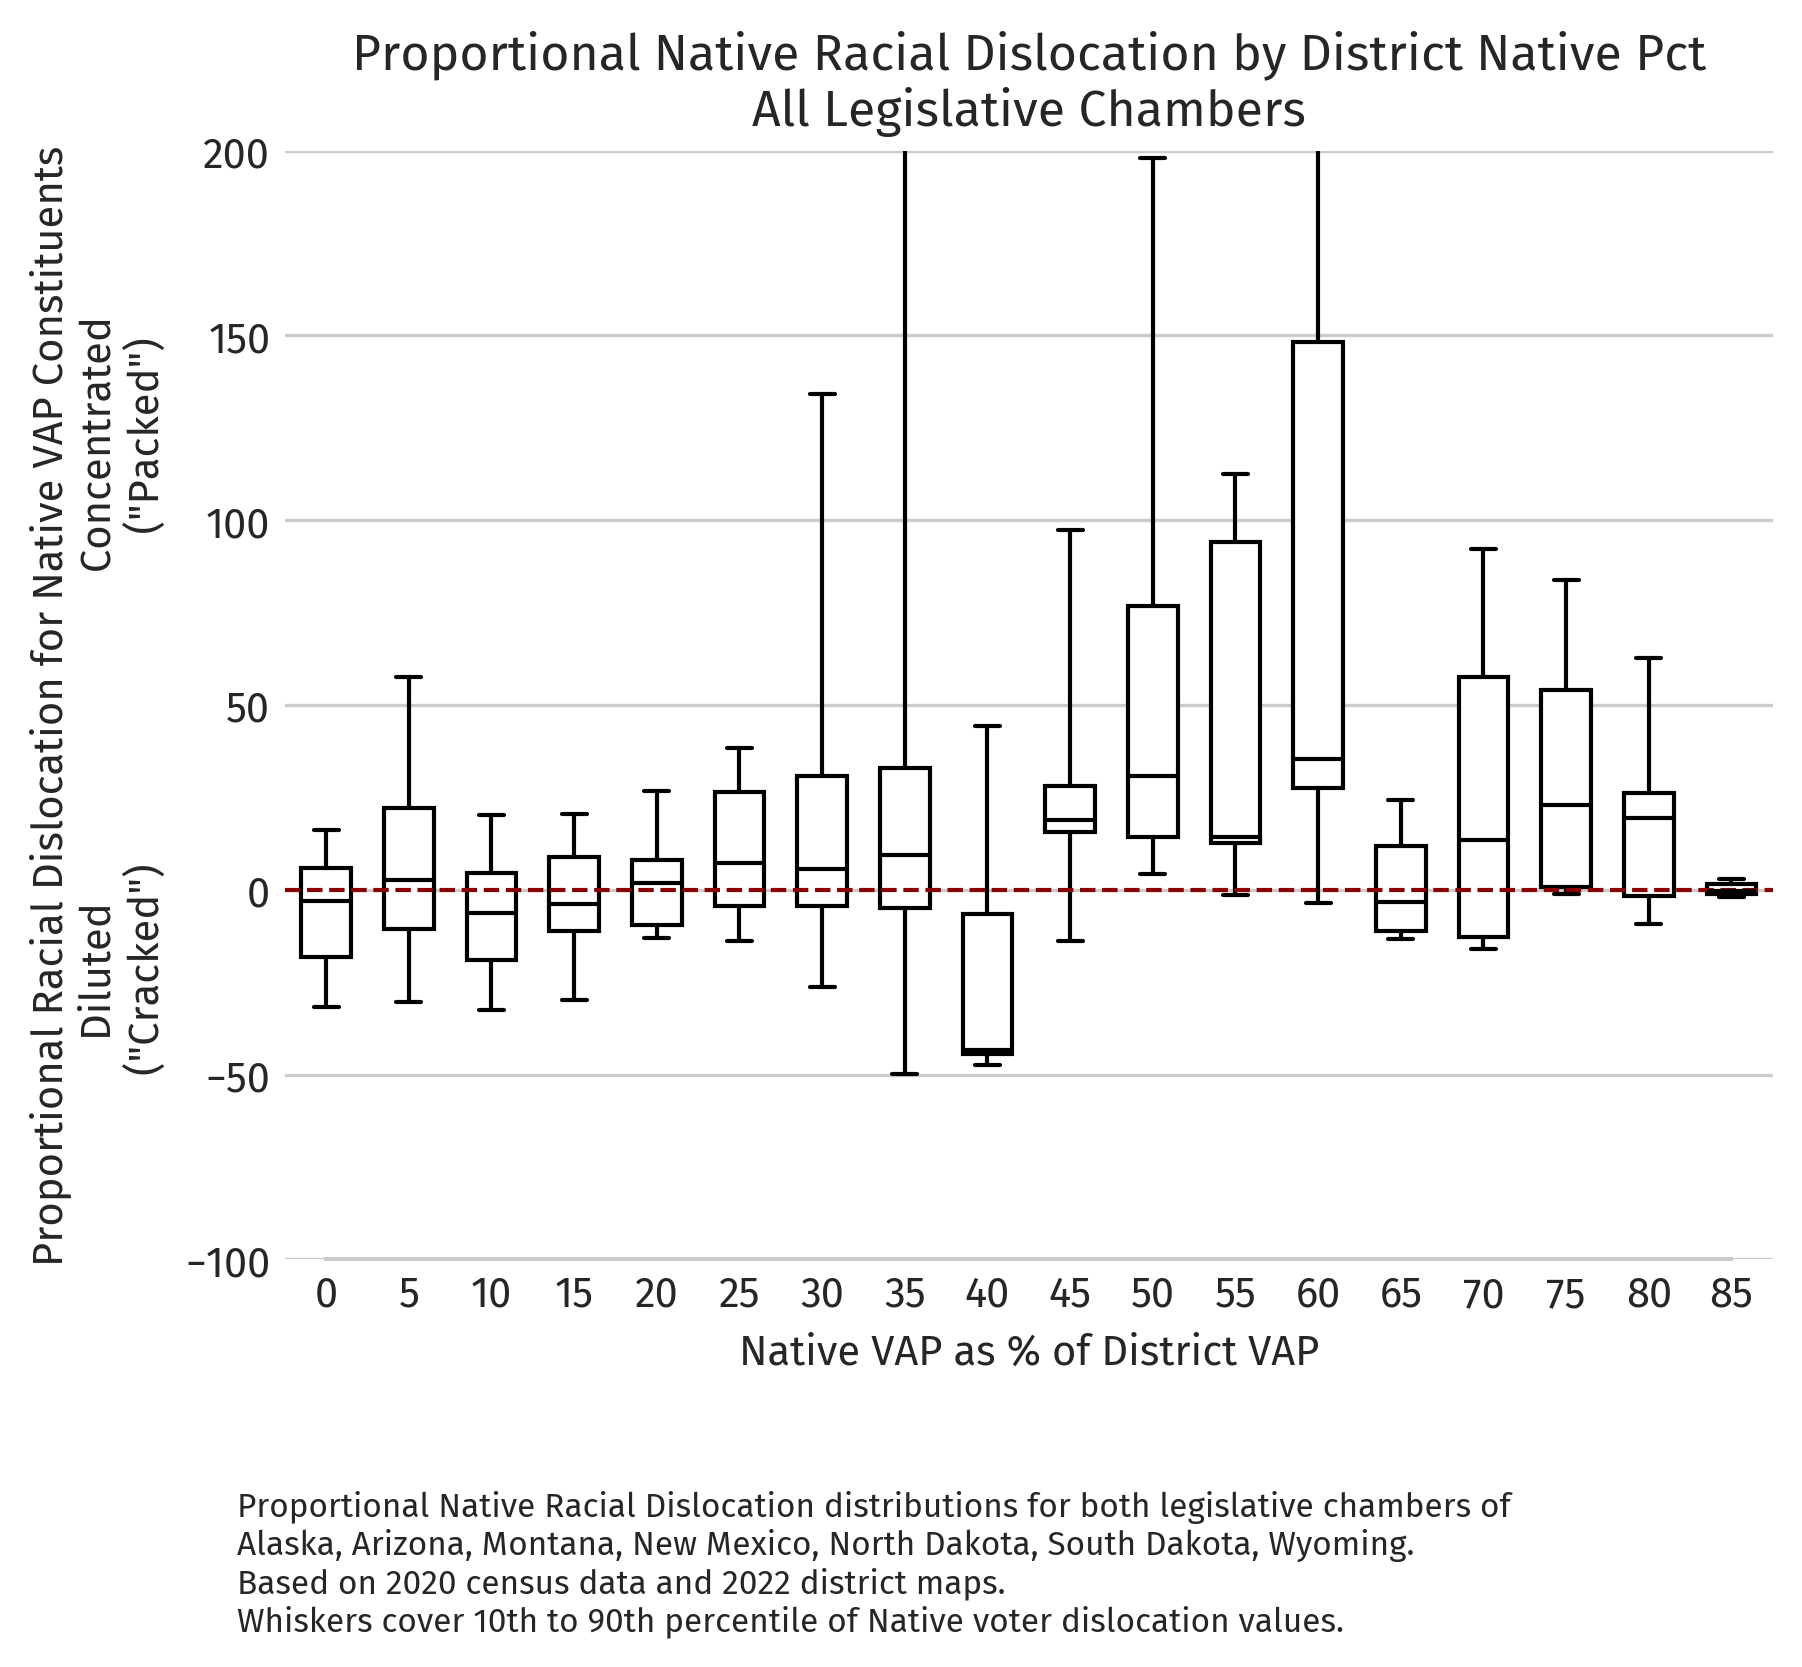
\includegraphics[width=0.8\textwidth]{figures/proportinal_dislocation_by_district_AI_map2023_census2020_chamberall.png}
  \caption{Proportional Dislocation by District NVAP (2022 districts)}
  \label{fig:Prop_Dislocation_Box_2020}
\end{figure}

Generally, with respect to majority-Native districts, proportional and absolute dislocation values both indicate significant packing, and generally among districts with a similar demographic composition.  It is in districts with smaller NVAP percentages that the two measures diverge somewhat: proportional dislocation values are higher in districts with small NVAP percentages.  This is because even small absolute dislocation values (for instance, a Native voter being in a 10\% NVAP district when their natural neighborhood has 12\% NVAP, resulting in an absolute difference of 2\%) can be significant when that difference is measured as a proportion of the NVAP percentage of the voter's district (2\% divided by 10\% = 20\%).



\end{document}